\documentclass{article} % For LaTeX2e
\usepackage[submission]{colm2025_conference}

\usepackage{microtype}
\usepackage{hyperref}
\usepackage{url}
\usepackage{booktabs}

\usepackage{lineno}
\usepackage{graphicx}
\usepackage{tcolorbox}
\usepackage{tikz}
\usetikzlibrary{positioning, fit, arrows.meta, shapes.geometric}
\usepackage{wrapfig}
\usepackage{colortbl} % For row coloring
\usepackage[T1]{fontenc}

% Algorithm formatting
\usepackage{algorithm}
\usepackage{algpseudocode}

\definecolor{darkblue}{rgb}{0, 0, 0.5}
\hypersetup{colorlinks=true, citecolor=darkblue, linkcolor=darkblue, urlcolor=darkblue}


\title{AutoLibra \protect
\includegraphics[height=1em]{figs/scale.png} \\ \textit{Metric Induction for Agents from Open-Ended Human Feedback}}

% Authors must not appear in the submitted version. They should be hidden
% as long as the \colmfinalcopy macro remains commented out below.
% Non-anonymous submissions will be rejected without review.

\author{Antiquus S.~Hippocampus, Natalia Cerebro \& Amelie P. Amygdale \thanks{ Use footnote for providing further information
about author (webpage, alternative address)---\emph{not} for acknowledging
funding agencies.  Funding acknowledgements go at the end of the paper.} \\
Department of Computer Science\\
Cranberry-Lemon University\\
Pittsburgh, PA 15213, USA \\
\texttt{\{hippo,brain,jen\}@cs.cranberry-lemon.edu} \\
\And
Ji Q. Ren \& Yevgeny LeNet \\
Department of Computational Neuroscience \\
University of the Witwatersrand \\
Joburg, South Africa \\
\texttt{\{robot,net\}@wits.ac.za} \\
\AND
Coauthor \\
Affiliation \\
Address \\
\texttt{email}
}

% The \author macro works with any number of authors. There are two commands
% used to separate the names and addresses of multiple authors: \And and \AND.
%
% Using \And between authors leaves it to \LaTeX{} to determine where to break
% the lines. Using \AND forces a linebreak at that point. So, if \LaTeX{}
% puts 3 of 4 authors names on the first line, and the last on the second
% line, try using \AND instead of \And before the third author name.

\newcommand{\fix}{\marginpar{FIX}}
\newcommand{\new}{\marginpar{NEW}}

\begin{document}

\ifcolmsubmission
\linenumbers
\fi

\maketitle

\begin{abstract}
The evaluation and optimization of language agents are often based on either
task success or heuristically designed metrics.
However, these approaches are either not fine-grained enough or require 
manual design of the metrics by experts.
We propose \emph{AutoLibra},
a system that transforms human feedback, 
\emph{e.g.} ``\textsf{If you find that the button is disabled, don't click it again}'',
or ``\textsf{This agent has too much autonomy to decide what to do on its own}''
into metrics evaluating similar failure and successful modes.
AutoLibra accomplishes this by first grounding the feedback in the agent's behavior,
clustering similar positive and negative behaviors,
and creating metrics that are ready to prompt LLM-as-a-Judge with
concrete examples and definitions. 
We propose two \emph{meta metrics} to evaluate how aligned a set of (induced) metrics
is with human open-ended feedback: ``coverage'' and ``redundancy''.
Through optimizing these meta metrics, we find that AutoLibra could
not only recover the \textbf{agent evaluation} dimensions heuristically proposed
in previous agent evaluation benchmarks, but also discover the ones that have been overlooked.
Beyond agent evaluation, we demonstrate two practical applications of
AutoLibra in \textbf{agent improvement}:
First, we demonstrate that the metrics extracted by AutoLibra serve
as better optimization targets than task success rate on two challenging text game tasks,
enhancing prompt engineering. 
Second, we show that AutoLibra can also interatively selects high-quality agent fine-tuning data
for web browsing. 
Our results suggest that AutoLibra can be a powerful tool for
evaluating and improving language agents.
\end{abstract}


\section{Introduction}

\begin{wrapfigure}[18]{r}{0.45\textwidth}
   \vspace{-40pt}
   \centering
   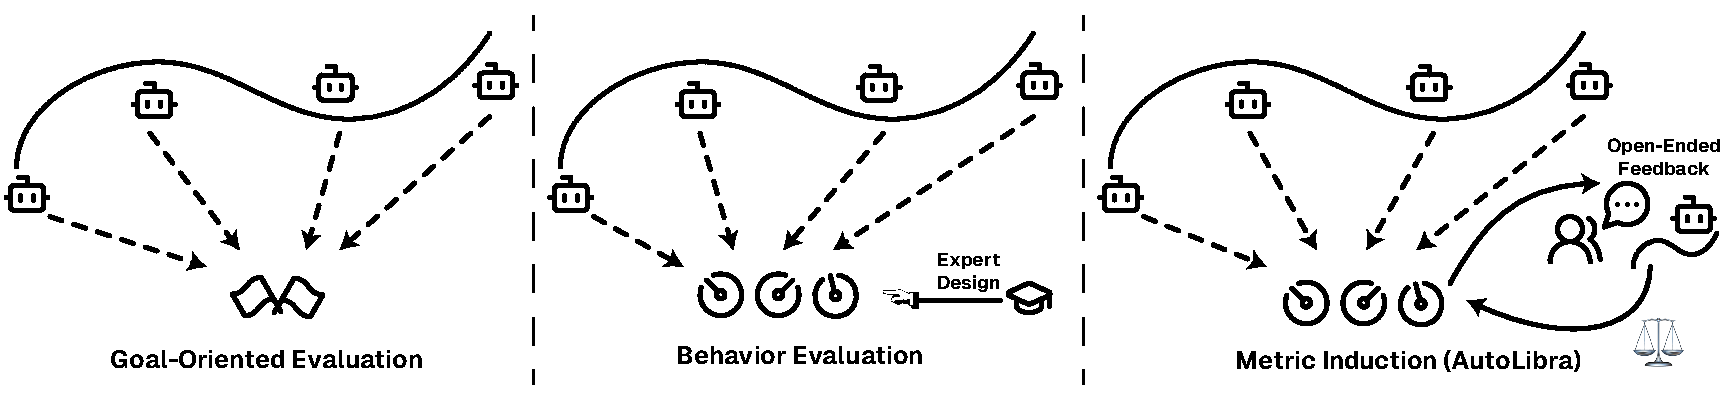
\includegraphics[width=0.45\textwidth]{figs/autolibra.pdf}
   \caption{AutoLibra provides behavioral evaluation on agent performance
    through automatic metric induction based on human feedback and agent trajectories.}
\end{wrapfigure}


Efficient human learners internalize open-ended feedback from others into self-regulation metrics
\citep{pintrich2002development,nicol2006formative}.
These metrics offer lenses for self-reflection on the
strengths and weaknesses of ourselves and ladders for self-improvement.
In this paper, we ask:
\textbf{can we automatically induce metrics to evaluate and improve language agents from natural language feedback?} 

   
The current evaluation of large language model (LLM) agents and reward modeling often fall
into two paradigms: (1) goal-oriented evaluation --
\emph{whether the agents have fulfilled the given task},
\emph{e.g.} benchmarks \citep{zhouwebarena,jimenezswe,chan2024mle,paglieri2024balrog} and reward
modeling approaches \citep{pan2024autonomous,chen2025scaling,choudhury2025process}
and (2) behavior evaluation -- \emph{how well the agents do on heuristically designed dimensions},
\emph{e.g.} social agent and human-agent interaction benchmarks \citep{zhousotopia,shao2024collaborative}
and agent failure mode analysis \citep{pan2025why,zhang2023effects,yang2023behavioral}. 
Goal-oriented evaluation is often designed to be verifiable through considering, but it is not fine-grained
or comprehensive enough to diagnose agents' behavior problems or find the bottlenecks for improvements \citep{yehudai2025survey}.  
While behavior evaluation complements it, it requires manual design of the metrics either based on top-down heuristics
\citep{zhousotopia}, or thematic analysis of the agent's behavior \citep{shao2024collaborative,pan2025why}.
This manual design process is often time-consuming and labor-intensive through expert annotations and classifications. 

In this paper, we introduce AutoLibra \protect
\includegraphics[height=1em]{figs/scale.png},
a metric induction method as a new agent evaluation paradigm 
that mitigates the limitations of the current evaluation paradigms.
This method offers behavior evaluation for agents, with the following advantages:
(1) it provides multi-dimensional behavior evaluation that is fine-grained but requires no manual design of metrics,
(2) it could be applied to different kinds of agents and tasks, and 
(3) the metrics are fully explainable and interpretable by humans.

Taking an inspiration from the code-theme steps of thematic analysis often conducted by human experts in social sciences \citep{braun2006using},
we design the Extraction process of AutoLibra as a two step process:
(1) \emph{grounding}: ground every aspect of the human feedback into a slice of the whole agent trajectory,
and (2) \emph{clustering}: cluster the aspects of all trajectories into multiple clusters of similar behaviors
that can be summarized into metrics. For example, in the context of web agents, the grounding step will
``\textsf{If you find that the button is disabled, don't click it again}'' into a slice of the agent trajectory
``\texttt{action: click[1234]} \texttt{obs: no change} \texttt{action: click[1234]}''. Similar slices where 
agents repeated interact with disabled elements could be clustered into a metric \texttt{repeated-interact-disabled}. 

The Evaluation process of AutoLibra is designed to meta-evaluate the LLM-as-a-Judge results
through matching the detected agent traits with human feedback aspects.


we design AutoLibra as a closed-loop system
that has an \emph{Extraction Step} which extracts metrics from human feedback and agent trajectories,
and an \emph{Evaluation Step} which meta-evaluates the LLM-as-a-Judge results
through matching the detected agent traits with human feedback aspects. 
Through these two steps, AutoLibra optimizes not only for metrics that represents humans' views on the
agents' behavior, but also for the metrics that are suitable for the LLM-as-a-Judge to produce human-aligned
evaluation results.

\begin{wrapfigure}{r}{0.7\textwidth}
    \centering
    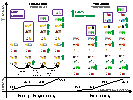
\includegraphics[width=0.7\textwidth]{figs/autolibra-teaser.pdf}
    \caption{Caption}
    \label{fig:enter-label}
\end{wrapfigure}

The Extraction Step of AutoLibra is designed to extract metrics from human feedback and agent trajectories.


With AutoLibra, we aim to answer the following research questions:
\begin{itemize}
    \item \textbf{RQ1:} Can LLMs serve as a proxy for humans when being used in agent behavior thematic analysis,
    behavior evaluation, and meta-evaluating the LLM-as-a-Judge results?
    \item \textbf{RQ2:} What are the differences between the metrics induced by AutoLibra and the behavior evaluation
    metrics designed by human experts?
    \item \textbf{RQ3:} Is AutoLibra useful for improving the performance of agents in different tasks by 
    providing fine-grained behavior evaluation for human agent engineers and agent learning algorithms?
\end{itemize}





\section{\texorpdfstring{AutoLibra 
\includegraphics[height=1em]{figs/scale.png}}{AutoLibra}}

To address the limitations of existing evaluation paradigms, AutoLibra \protect
\includegraphics[height=1em]{figs/scale.png} is designed to
meet the following desiderata: (1) \emph{induced from agent behavior}: This ensures that metrics are grounded in agent trajectories rather than predefined by human experts, (2) \emph{self-validating}: Allows choosing minimal set of metrics that cover unseen human feedback with sufficient abstraction to be useful across different tasks, and (3) \emph{generalizable}: Applicable to various agent environments, independent of domain-specific design.

Based on feedback data collected from humans (\S\ref{sec:collecting-human-feedback}), AutoLibra achieves these desiderata through a closed-loop pipeline
consisting of two processes: \textbf{Induction Process} that converts agent behaviors and corresponding feedback into metrics, (\S\ref{sec:induction_process}) and \textbf{Evaluation Process} that predicts ratings and quality of new agent behaviors on the induced metrics (\S\ref{sec:evaluation_process}). 


\subsection{Collecting human feedback}
\label{sec:collecting-human-feedback}
In this paper, we use human feedback from two groups: (1) End-users -- for agents that interact directly with humans, we use the feedback from the users who interact and converse with the agents. CoGym \citep{shao2024collaborative}
is the environment that belongs to this category, and we use the user comments collected in their study, resulting
in 197 trajectories with feedback. (2) Experts -- for agents that
do not directly interact with humans, we use the feedback from human annotators (five authors in this paper) who observe agent trajectories. All other environments belong to this category, these being Sotopia \citep{zhousotopia}, WebArena \citep{zhouwebarena}, WebVoyager \citep{he2024webvoyager}, Baba-is-ai \citep{cloos2024babaaibreakrules}, and MiniHack \citep{samvelyan2021minihackplanetsandboxopenended}. For each trajectory, we collect only one element of feedback; feedback is given based on the complete agent trajectories.\footnote{While in theory we can leverage feedback on specific steps to achieve better feedback grounding and multiple feedback for single trajectory, we leave it as future work.}

\begin{wrapfigure}[17]{r}{0.4\linewidth}
  \vspace{-10pt}
  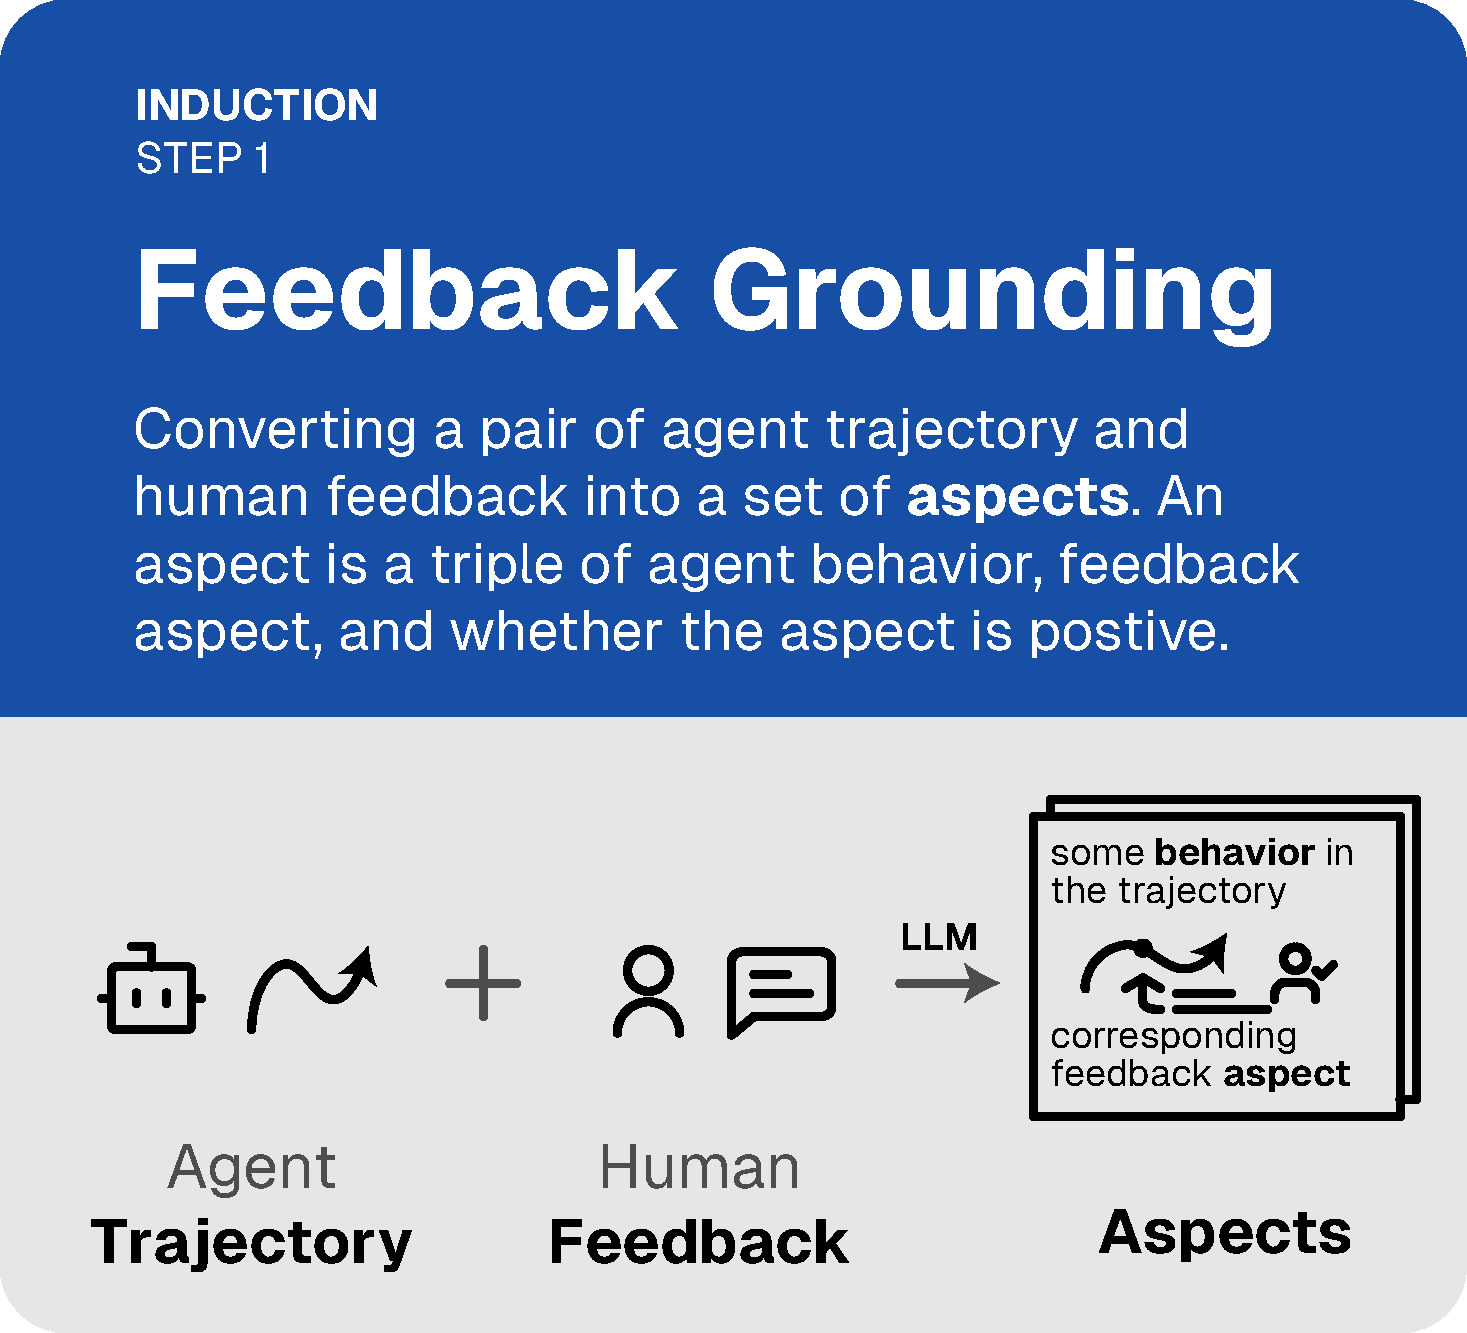
\includegraphics[width=\linewidth]{figs/autolibra_step_1.pdf}
  \vspace{-10pt}
  \caption{Feedback Grounding}
  \label{fig:feedback_grounding}
\end{wrapfigure}
Annotators are instructed to explicitly indicate the aspects of agent behavior that they classify as good or bad,
and to avoid general comments such as \textsf{"The agent is good at solving the task"}.
The annotators can also choose from a TTY (TeleTYpewriter) or a web interface; in both cases the annotator is provided with the agent's task
and then view the agent's observation and actions step by step, in text form. \footnote{While viewing screenshots is standard for web navigation tasks, we keep the observation format consistent across agents and humans to encourage more grounded feedback.}
For multi-agent tasks, we annotate each agent's trajectory in a given interaction separately. For Sotopia \citep{zhousotopia}, WebArena \citep{zhouwebarena},
and WebVoyager \citep{he2024webvoyager}, we annotate 100 trajectories of agents based on GPT-4 \citep{achiam2023gpt} with feedback for each dataset. For experiments in \S\ref{sec:ladder} we annotate 18 trajectories for each dataset in each
iteration. The annotation process is fast: Human annotators spend less than 5 minutes to provide feedback for each trajectory; \S\ref{sec:lens}, we randomly hold out 20\% of the trajectories for validation.

% \begin{figure}
%     \centering
%     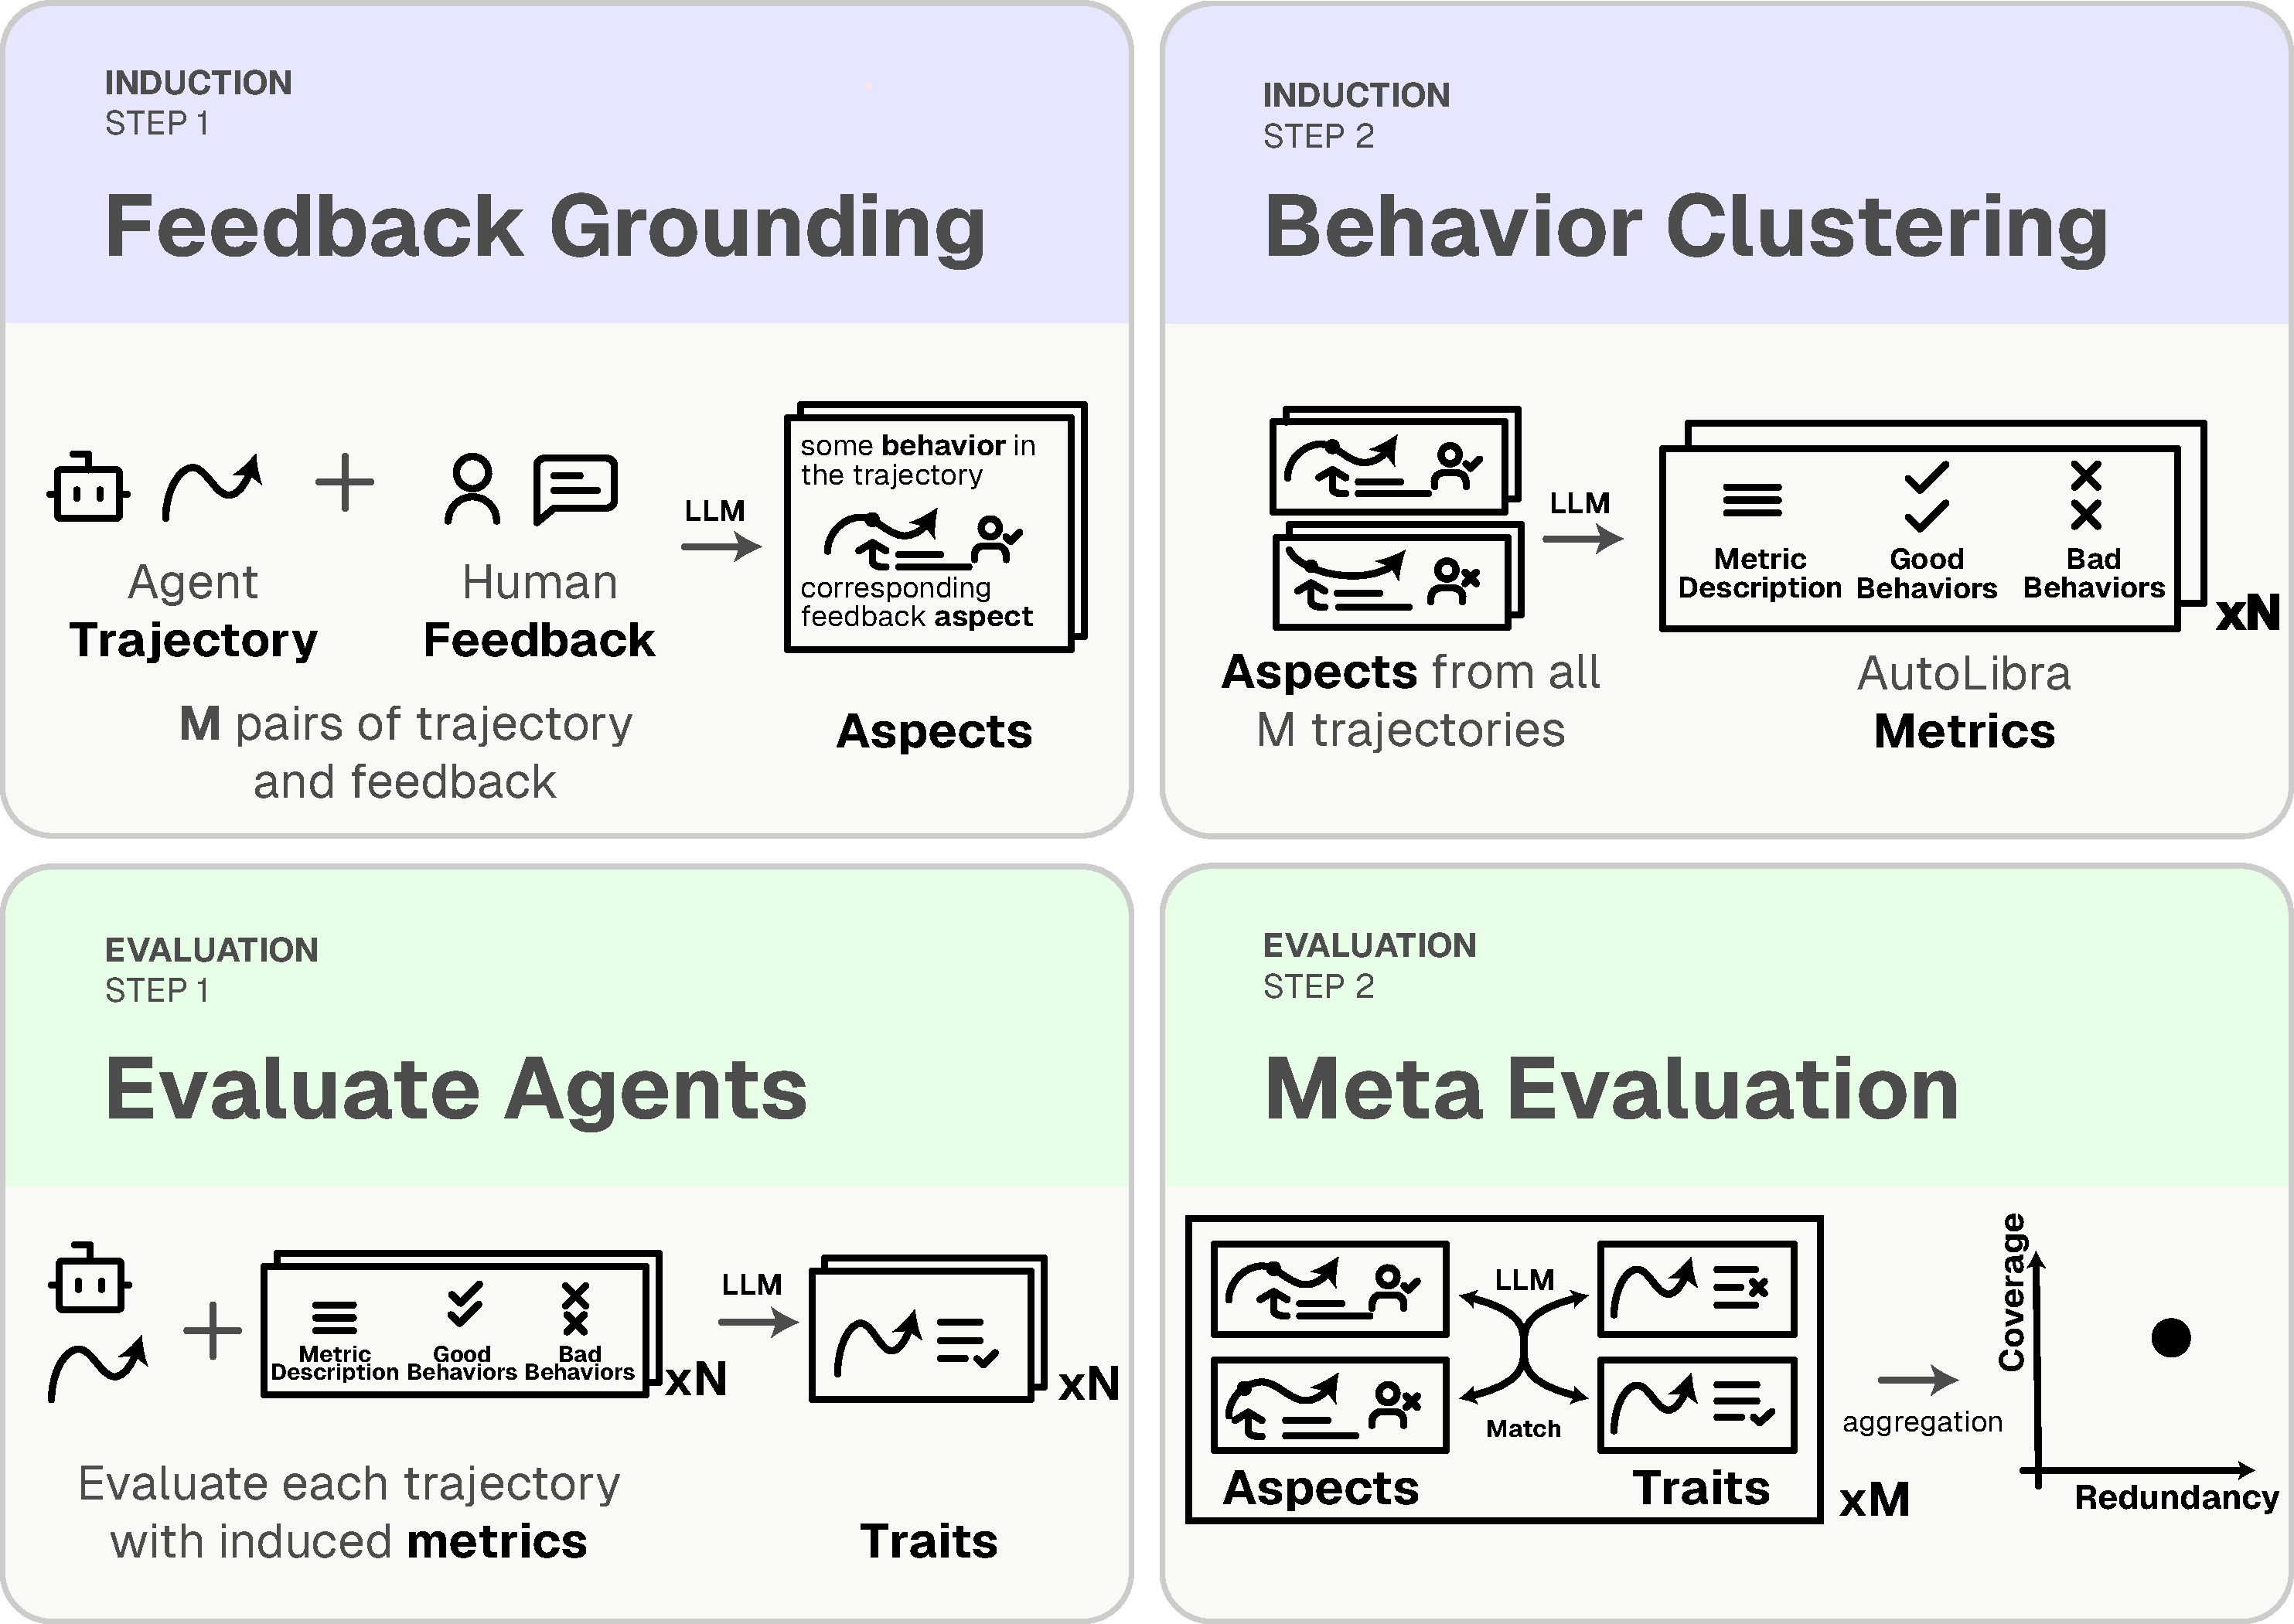
\includegraphics[width=\linewidth]{figs/autolibra_pipeline_v2.pdf}
%     \caption{Caption}
% Caption    \label{fig:enter-label}
% \end{figure}


\subsection{Induction Process: agent trajectories and human feedback $\rightarrow$ evaluation metrics}
\label{sec:induction_process}

\paragraph{Feedback Grounding}
The feedback of human annotators can contain multiple aspects; e.g. \textsf{``AI agent was pretty good
at giving me a consistent itinerary and vacation plan, although it froze on the last couple of minutes.''},
%\diyi{are all feedback from cogym? the current writeup is confusing and easily get readers to think about the feedback is from cogym only. if not, we need to add a few sentences saying how feedback is achieved, and how easy it is for humans to provide such feedback. otherwise, if this is something taking a lot of time, why do we want to use it?} 
collected from human annotators in CoGym \citep{shao2024collaborative}, contains a positive aspect
about the agent's ability to generate a consistent itinerary, and a negative aspect about the agent freezing
at the end. Here we define an \emph{aspect} as a triple $(\texttt{behavior}, \texttt{feedback}, \texttt{sign})$.
In the positive aspect of the previous example, the \texttt{behavior} is the agent's actions to create
a 20-day itinerary for the Maldives, the \texttt{feedback} is that the created itinerary is consistent and the \texttt{sign} is positive. This grounding procedure is similar to the coding procedure in thematic analysis by humans.



Illustrated in Fig. \ref{fig:feedback_grounding}, in this step, we feed the trajectory and the feedback into the LLM (we use GPT-4o \citep{openai2024gpt4ocard} 
as it yields good results in our pilot experiments) and prompt the LLM with the following instructions:
(1) break down the feedback into bullet points; (2) for each bullet point, find the corresponding
part of the trajectory to which the feedback refers. Finally, we use constrained decoding to force GPT-4o
to output the aspects in the previous format. In our experiments, we find that on most datasets, for each
trajectory, the LLM can generate one to five aspects, with a mean of one to two aspects.


\paragraph{Behavior Clustering}
\begin{wrapfigure}[16]{l}{0.4\linewidth}
  \vspace{-10pt}
  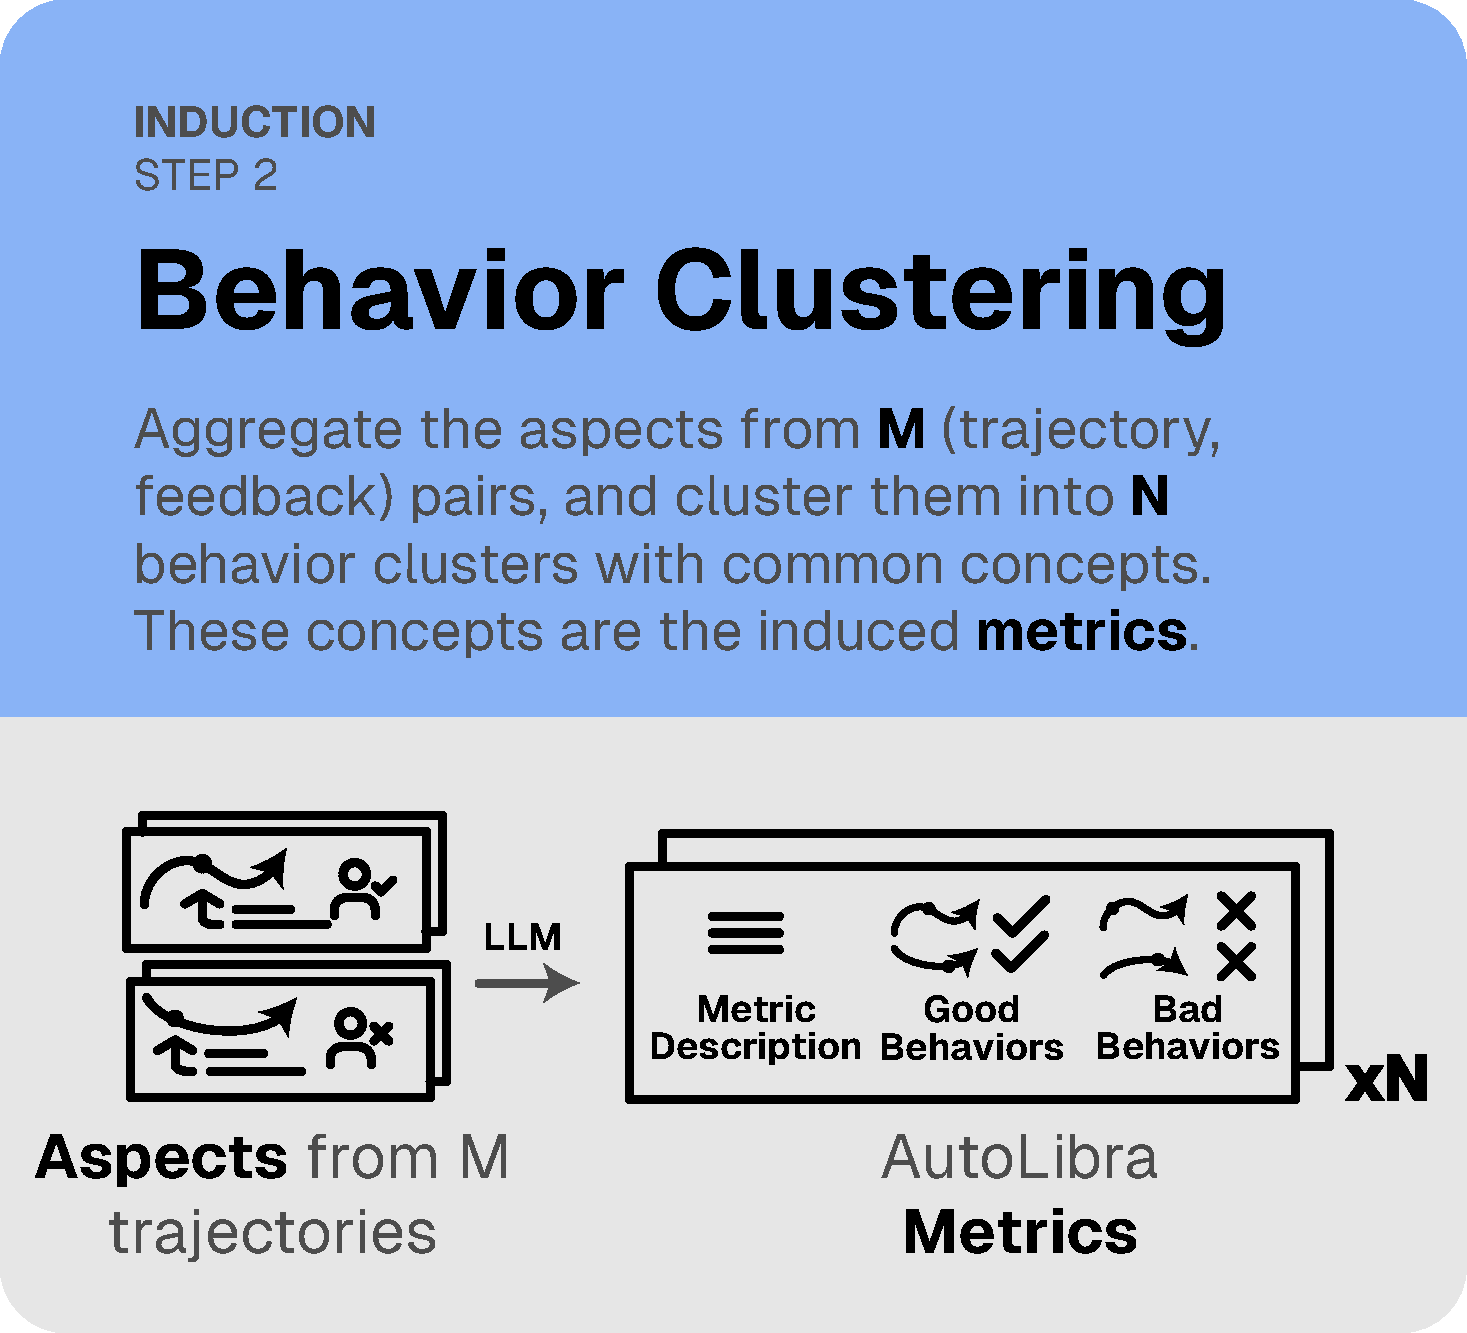
\includegraphics[width=\linewidth]{figs/autolibra_step_2.pdf}
  \vspace{-10pt}
  \caption{Behavior Clustering}
  \label{fig:behavior_clustering}
\end{wrapfigure}
The second step of the extraction process is to group the aspects into $N$ metrics.
To illustrate this step, we consider another example in the same dataset
\textsf{``The AI responds quickly to write and run the Python script``} where
the \texttt{behavior} is the agent's action to quickly write and run a Python script, the \texttt{feedback}
is that the agent responds quickly, and the \texttt{sign} is positive. Although this aspect is a positive aspect,
it reflects the same dimension of the agent's behavior as the previous negative aspect, with an opposite value.
Each \emph{metric} is a cluster of aspects, with a definition summarizing the criteria of positive behaviors, a list of positive behavior examples, and a list of negative behavior examples. This clustering procedure
is similar to the theme induction step in thematic analysis.

However, clustering similar agent behaviors together is challenging for statistical clustering methods.\footnote{
    In preliminary experiments, we tried to use K-means clustering on the aspect vectors generated by \texttt{text-embedding-3-large},
    but the clusters are mostly based on tasks and not on the behaviors.
}
Inspired by LLM-based semantic clustering and concept induction methods \citet{viswanathan2024large,lam2024concept}, we prompt an LLM (o3-mini high\footnote{https://openai.com/index/openai-o3-mini/}, as it produces the most accurate coverage and redundancy scores as evaluated later) 
to cluster the aspects into metrics. 
As illustrated in Fig. \ref{fig:behavior_clustering},
we gather all the aspects of $M$ trajectories
and cluster into $N$ metrics, where $N$ is a parameter set through the optimization process (\S\ref{sec:metric-optimization}).
We provide the LLM with the following instructions:
\emph{The granularity of the grouping should be minimal; only very similar behaviors are grouped together; but don't limit to one particular website or one particular character}, which empirically
makes the metrics more concrete but still applicable across different tasks.


\subsection{Evaluation Process: evaluating agents and the quality of the induced metrics}
\label{sec:evaluation_process}

\paragraph{Evaluating agents with induced metrics}
LLM-as-a-Judge \citep{zheng2023judging},
or more broadly, model-based evaluation
\citep{zhang2019bertscore,celikyilmaz2021evaluationtextgenerationsurvey}
is a method to use machine learning models to evaluate the output of other machine learning models.
The success of LLM-as-a-Judge depends on the gap between the difficulty of evaluation or verification and
that of generation and action. 
In agentic tasks, this gap is often large, as the policy model must perform multiple steps in decision-making, while the evaluation model must only
classify the trajectories, which make LLM-as-a-Judge widely used \citep{zhouwebarena,he2024webvoyager,zhousotopia}.
In AutoLibra, we employ LLM-as-a-Judge to
evaluate the agent trajectories configured with the induced metrics. However, LLM-as-a-Judge
can be replaced by any other evaluation methods implementing the induced metrics;
\emph{e.g.} an \texttt{interact-valid-element} metric
could be evaluated by a rule-based evaluator that checks if the agent
interacts with valid elements on the webpage. Wenote that AutoLibra could be used with other evaluation methods, such as
programmatic evaluation \citep{maeureka}; we leave generating programs for the induced metrics for future work.

\begin{wrapfigure}[16]{r}{0.4\linewidth}
  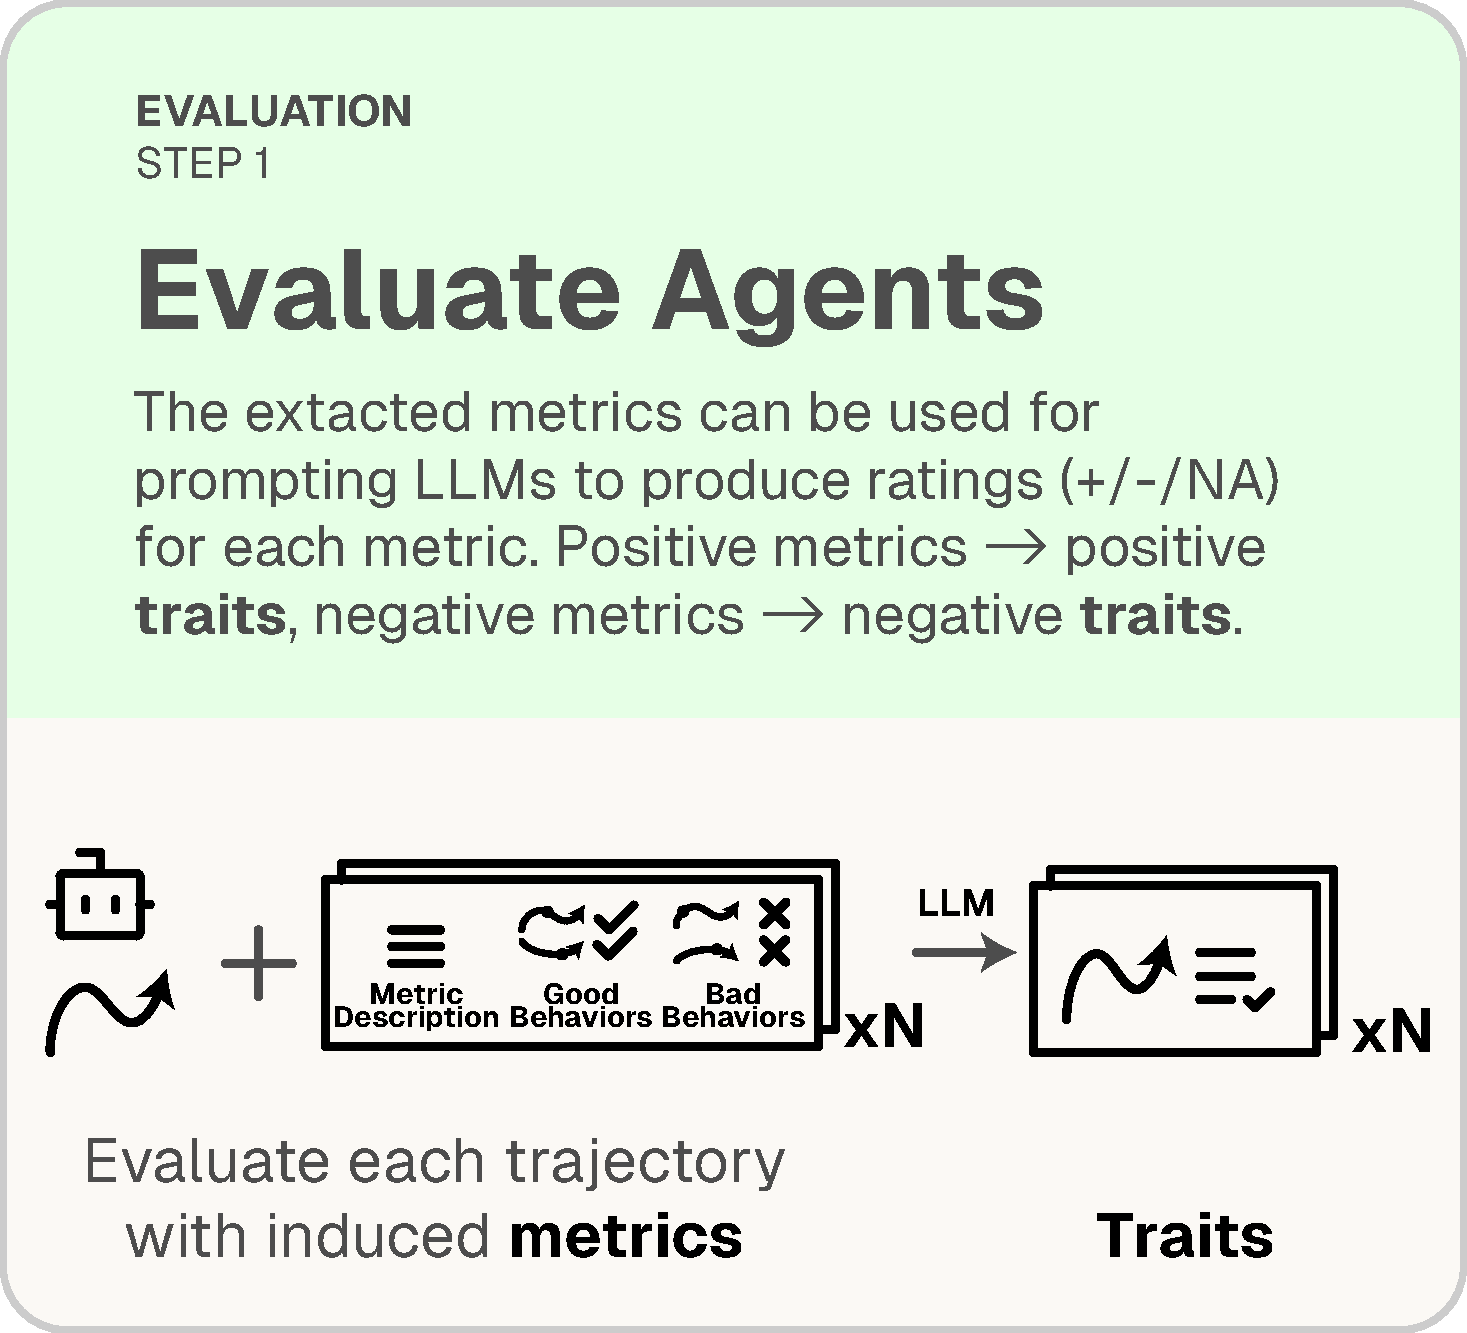
\includegraphics[width=\linewidth]{figs/autolibra_step_3.pdf}
  \vspace{-10pt}
  \caption{Evaluating agents with \\ induced metrics}
  \label{fig:llm_as_a_judge}
\end{wrapfigure}
As illustrated in Fig. \ref{fig:llm_as_a_judge}, taking the induced metrics as input, an LLM (we use o3-mini medium,
as it provides similar results in this step to o3-mini high) is prompted to rate the agent trajectories to \{+ 1, -1, N/A\} for each metric. For an agent trajectory, the metrics labeled +1 are
the positive \emph{traits}, and the ones labeled -1 are the negative \emph{traits}. When we calculate the scores of
the metrics, we use the ratio of agent trajectories rated as positive
to the ones that are rated as positive or negative, ignoring those rated as N/A,
since not all metrics are applicable to all trajectories
(some metrics like \texttt{valid-search-terms} are only applicable when the task
involves searching). 


\paragraph{Meta evaluation}
The last component of the loop is the meta-evaluation, i.e. evaluating the evaluation metrics induced by AutoLibra.
This step matches the traits detected by the LLM-as-a-Judge with aspects
grounded from the human feedback. The goal is to verify whether (1) the induced metrics cover the behaviors the human annotators care about, and (2) LLM-as-a-Judge can produce
accurate evaluation results based on the induced metrics. In the previous example,
if the \texttt{respond-promptly} is extracted as a metric, and the LLM-as-a-Judge
has the same opinion as the human annotators, then this aspect is considered as successfully covered.
If either a similar metric was not extracted, or the LLM-as-a-Judge assigns a different score,
then this aspect is considered as not covered.

\begin{wrapfigure}[15]{l}{0.4\textwidth}
  \vspace{-10pt}
  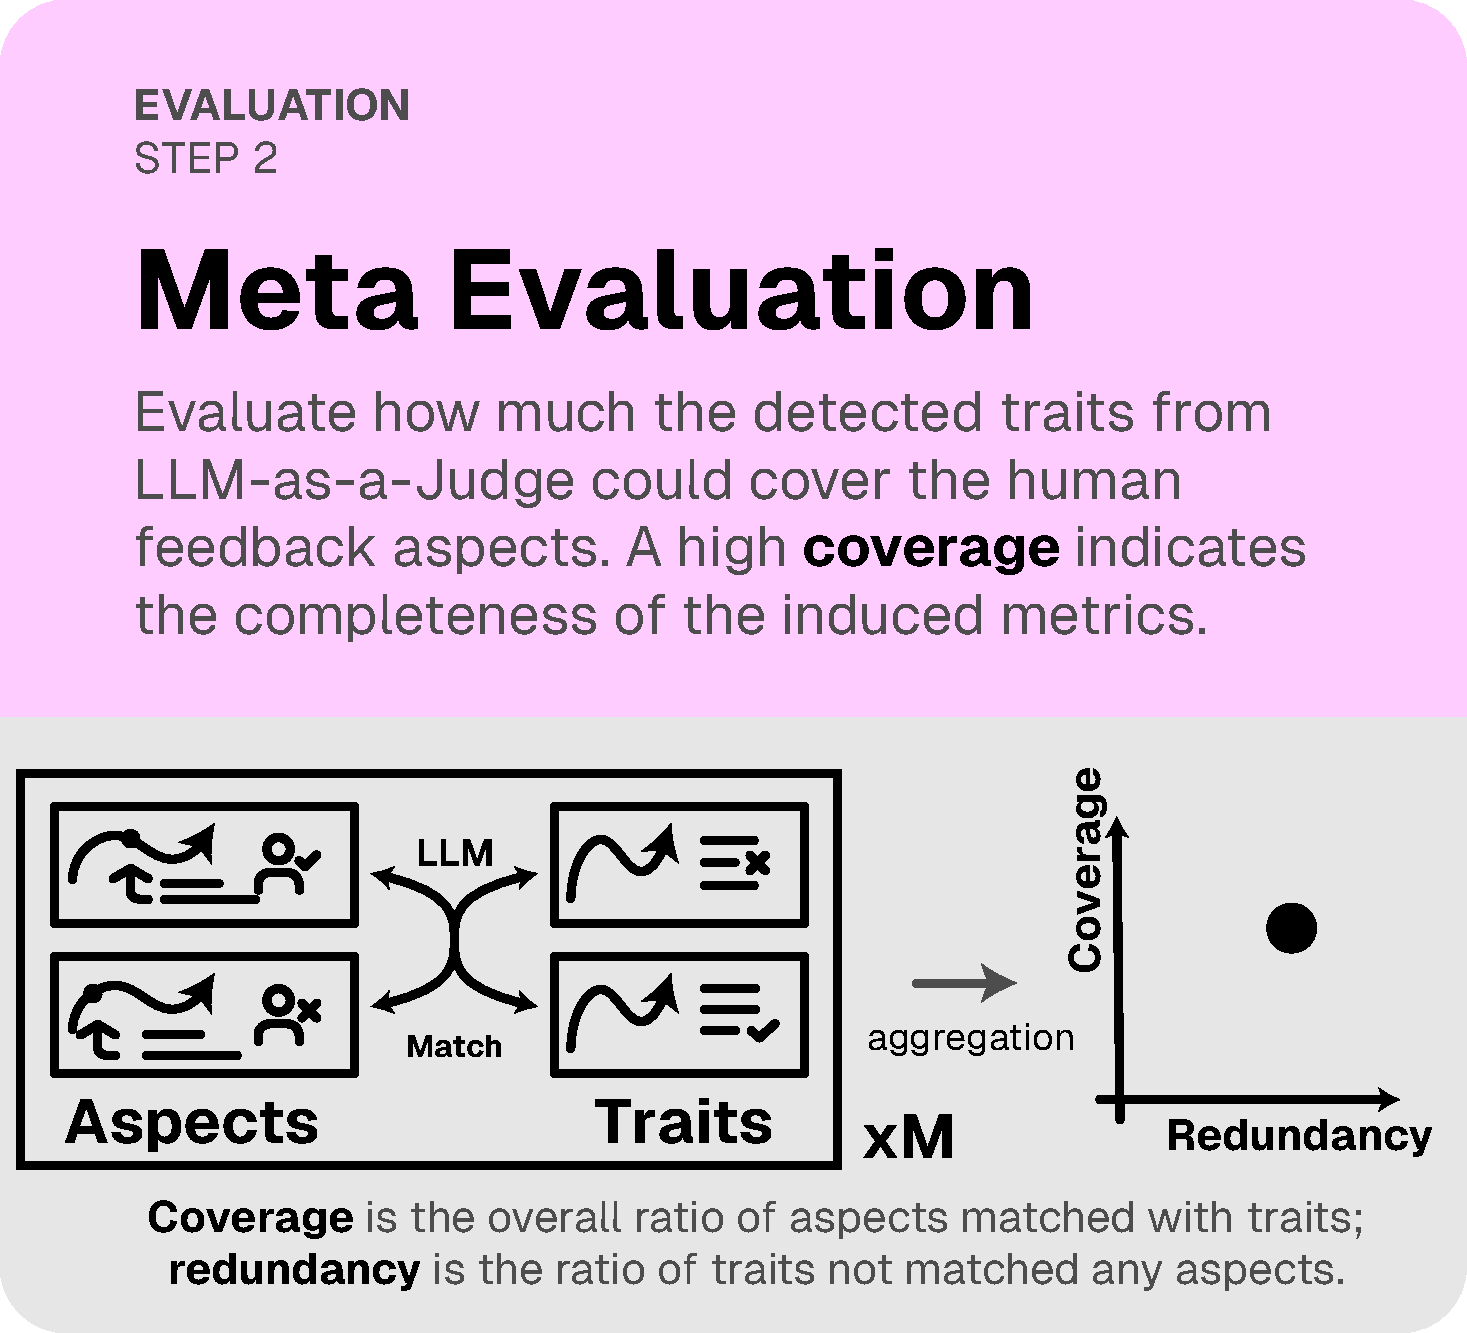
\includegraphics[width=\linewidth]{figs/autolibra_step_4.pdf}
  \vspace{-10pt}
  \caption{Meta evaluation}
  \label{fig:meta_evaluation}
\end{wrapfigure}
As illustrated in Fig. \ref{fig:meta_evaluation}, we perform meta-evaluation for each trajectory-feedback pair by classifying the aspects into positive and negative aspects, classifying
traits into positive and negative traits based on rating, then matching the positive aspects with positive traits
and the negative aspects with negative traits. 
We prompt an LLM (we use GPT-4o \citep{openai2024gpt4ocard}) with a list of aspects and another list of traits
and ask the LLM to find the best matching trait for each aspect or decide that there is no matching trait.
The \emph{coverage} of the whole dataset is calculated as the proportion of aspects of all instances that have a matching trait,
and the \emph{redundancy} is calculated as the proportion of traits of all instances that have not been matched with any aspect.

\section{Optimizing and validating AutoLibra \protect
\includegraphics[height=1em]{figs/scale.png}}
AutoLibra is designed to be self-validating through the evaluation process, which allows us to search the optimal set of metrics that cover the human opinion the best (\S\ref{sec:metric-optimization}). 
This optimization process can also be applied iteratively throughout the agent improvement process. As the agent is optimized, new metrics can be added to existing metrics (\S\ref{sec:iterative-induction}), which is similar to how unit tests are kept throughout software development to prevent new features from interfere with existing features. 
In the last part of this section, we study the alignment between each step of AutoLibra and human judgment. 


\subsection{Metric Optimization}
\label{sec:metric-optimization}

\begin{figure}[!t]
    \centering
    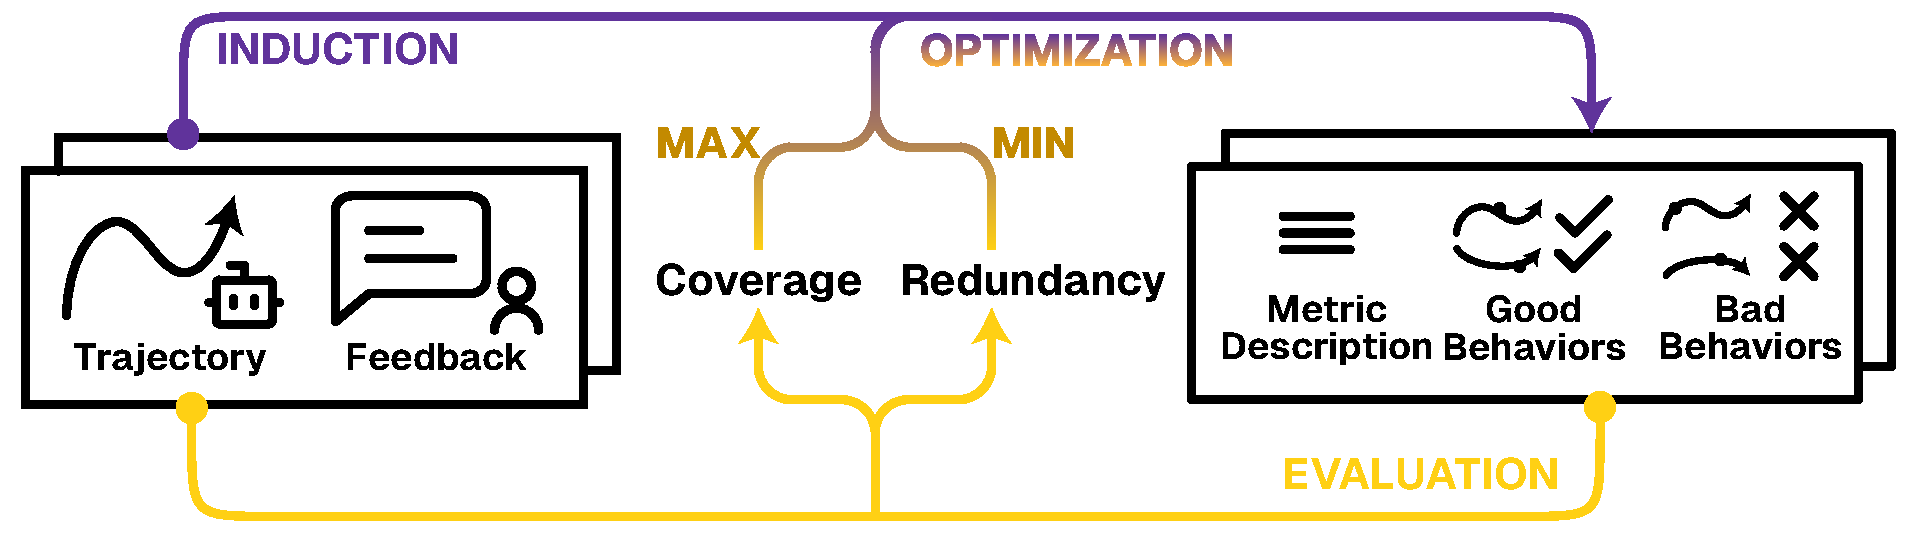
\includegraphics[width=0.8\linewidth]{figs/autolibra_optimization.pdf}
    \caption{Metric optimization: optimizing the induction process through maximizing the coverage while minimizing redundancy of the metrics, calculated via the evaluation process.}
    \label{fig:autolibra_optimization}
\end{figure}


As illustrated in Fig. \ref{fig:autolibra_optimization}, we optimize the metric induction process to maximize \textbf{coverage} and minimize \textbf{redundancy}.
Among the two, we prioritize coverage of the metrics to provide a comprehensive evaluation of the agent behavior, while minimizing overlap within the metrics to avoid redundancy, thus maximizing the utility of induced metrics.
To optimize for this objective, we generate 20 different sets of metrics, with $N$ ranging from 4 to 13,
and calculate the coverage and redundancy of the metrics in human feedback.
\begin{wrapfigure}[27]{r}{0.6\textwidth}
\vspace{-10pt}
    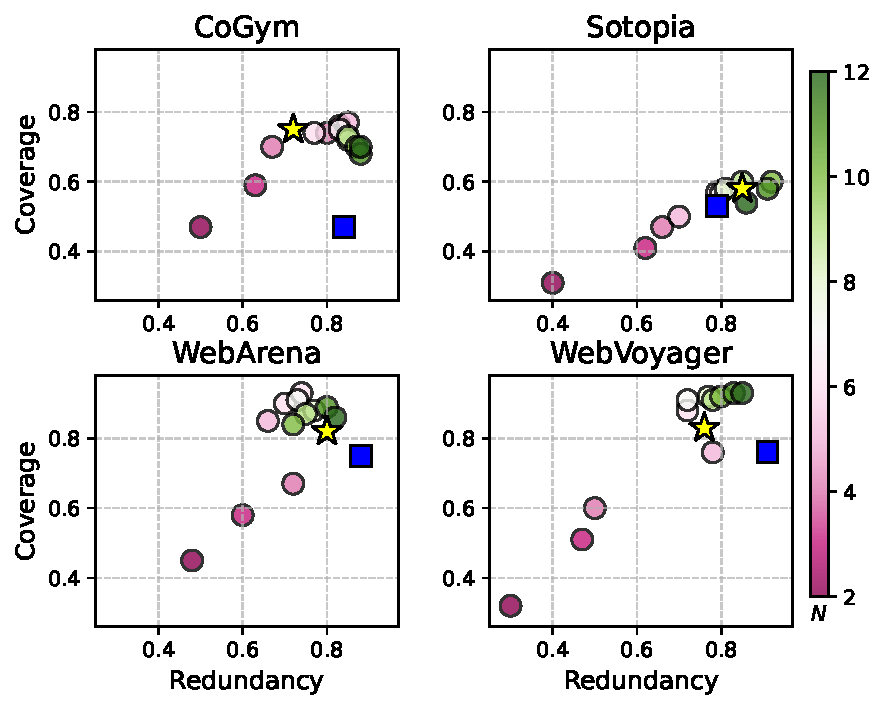
\includegraphics[width=0.6\textwidth]{figs/four_datasets_grid.pdf}
    \vspace{-15pt}  
    \caption{Coverage and redundancy of AutoLibra metrics on four agentic datasets. Circles indicate coverage and redundancy for different induced metrics; stars indicate the the best metrics' coverage and redundancy on held-out human feedback; squares show an ablation test, indicating the effect when good and bad behavior examples are removed from metrics, demonstrating the criticality of concrete behavior examples}
    \label{fig:coverage-redundancy}
\end{wrapfigure}
We then select metrics with a coverage of at least the highest coverage minus 1\%,
and the lowest redundancy.
This is performed iteratively, by resetting the range of $N$ to the number of metrics selected
previously $\pm$2, repeating until the coverage and redundancy
of the selected metrics converge, normally within 3 iterations.
While this optimization process is simple, experiments with various other optimization
strategies, including genetic algorithms and iterative clustering saw none of them
yield better results than the simple strategy.
Fig. \ref{fig:coverage-redundancy} shows the highest coverages of the metrics of size $N$, which converge around $N=6$ to $10$ depending on the datasets. The best coverage on Sotopia \citep{zhousotopia} is the lowest among all four datasets, $60\%$, likely due to the diversity of the tasks in the dataset, while coverage on WebArena \citep{zhouwebarena} and WebVoyager \citep{he2024webvoyager} are the highest, $88\%$. We also find that the coverage of the held-out trajectories is only slightly worse ($<5\%$) than the trajectories we use to induce the metrics, which is expected since we use the exact examples extracted from the latter. Lastly, we show that the good and bad behaviors are crucial in the metrics, dropping which resulting in up to $30\%$ coverage decrease (on CoGym \citep{shao2024collaborative}).



\subsection{Iterative Metric Induction}
\label{sec:iterative-induction}
When applying AutoLibra to agent optimization, we can iteratively induce new metrics, as agents develop new failure modes or new behaviors as they improve, which is useful for tracking agents' progress across different iterations.\footnote{Alternatively, a new set of metrics can be induced from scratch for each iteration -  in practice, we do not find that this results in any coverage loss, but we choose the former method for consistency} 
%For example, in the Baba-is-AI task \citep[\S\ref{sec:Baba-Is-AI}]{cloos2024babaaibreakrules}, the agent initially fails to recognize the win condition and acts randomly; after the agent improves with an in-context example in the prompt, the agent starts to follow existing win conditions, but fails to construct new win conditions. This was not mentioned in human feedback before the agent improvement, since the agent was too random to even reach the stage where constructing new win conditions is possible. Therefore, in the second iteration, a new metric \texttt{win-rule construction} should be induced to provide a new signal for further optimizing the agent.

%\diyi{did we do this, or is the below only a comment?}}

To do this, we modify the behavior clustering step, by providing the LLM with the existing metrics
and their definitions, and ask the LLM not to change the definitions of the existing metrics, 
to only add new behaviors to the existing metrics, and add new metrics if necessary.
We apply the same optimization strategy as in the metric optimization step
ensure the newly induced metrics cover emerging behaviors and do not overlap with existing metrics.

\subsection{How aligned are the steps in AutoLibra with human judgment?}
Since AutoLibra uses LLMs in each step, we first ask whether LLM outputs are reliable or aligned with human judgment. 
To measure the alignment of AutoLibra metric induction with human judgment, we validate the feedback grounding, agent evaluation, and meta evaluation steps by having human experts manually review each step (with exception of the behavior clustering step, as it is prohibitively time-intensive for human annotators to
process and cluster more than 400 aspects), scoring (1/0) based on whether they agree with the outcomes of each iteration. The coverage and redundancy scores, in combination with the validation results of the other steps in the loop, thus serve as an indirect validation for the behavior clustering step.
Table \ref{tab:validation} shows the agreement rate of human annotators in AutoLibra steps. 
It should be noted that these tasks are significantly different; e.g., grounding for WebVoyager \citep{he2024webvoyager} is challenging
due to the length and wide action space of the trajectory, and LLM-as-a-Judge for Sotopia \citep{zhousotopia} is
difficult due to the complexity of the evaluation of social interactions. Our results show that the majority (significantly over 85\%) of results in AutoLibra are reliable according to human validation. 

\begin{table}[!t]
    \centering
    \small
    \begin{tabular}{cccccc|c}
        \toprule
        Steps & CoGym & Sotopia & WebArena & WebVoyager & Baba-is-AI & Average  \\
        \midrule
        Grounding & 0.95 & 0.95 & 0.98 & 0.93 & 0.93 & 0.95 ($\pm 0.03$) \\
        LLM-as-a-Judge & 0.90 & 0.85 & 0.95 & 1.00 & 0.90 & 0.92 ($\pm 0.04$) \\
        Meta-Evaluation & 0.98 & 0.90 & 0.85 & 0.83 & 0.95 &  0.90 ($\pm 0.04$) \\
        \bottomrule
    \end{tabular}
    \caption{
        The ratio of instances marked as fully correct in human validation. For each step and each task, we randomly sample 40 instances to reach a relatively small confidence interval of $0.04$ and ask human annotators to label them as completely correct
        or not. Although the agreement scores vary across tasks and steps, the average agreement for each step and dataset is above 0.85 significantly. 
}
    \label{tab:validation}
\end{table}

%\diyi{S2 would benefit from a bit reorg. if you want, you can put 2.1, 2.2, 2.3 into one new subsection "Introducing AutoLibra (Pipeline)", and then use them as subsubsections; i would merge 2.4 and 2.5 as a second new subsection "Optimizing AutoLibra" and put the original 2.4 and 2.5 as subsubsections within it, to create more logic structures. i would move 2.6 to S3 as how you set up the initialization for using autolibra, etc.}

\section{\texorpdfstring{AutoLibra as a lens 
\includegraphics[height=1em]{figs/microscope.png}: agent evaluation with AutoLibra}{AutoLibra as a lens: agent evaluation with AutoLibra}}
\label{sec:lens}

In this section, we use AutoLibra as a lens to provide grounded, behavior-salient insights into agent trajectories. In three data sets, CoGym \citep{shao2024collaborative}, Sotopia \citep{zhousotopia}, and WebVoyager \citep{he2024webvoyager}, we compare induced metrics with heuristically proposed evaluation dimensions and failure modes summarized by the authors. We find that AutoLibra can discover more concrete metrics than heuristically defined categories, and novel metrics that are overlooked by experts. 

\begin{table}[!h]
\centering
\begin{tabular}{ll}
    \toprule
    AutoLibra\protect
\includegraphics[height=1em]{figs/scale.png}-induced metrics & CoGym failure categories\\\midrule
    \multicolumn{2}{c}{Matched metrics and categories}\\\midrule
    \textit{Responsiveness and Efficiency} (75\%) & \textit{Communication} (65\%) \\
    \emph{Communication Clarity and Notification} (8\%) & \textit{Communication} (65\%)\\
    \textit{Instruction Adherence and Follow-Through} (24\%) & \textit{Situational Awareness} (40\%)\\
    \textit{Iterative Refinement and Adaptability} (47\%) & \textit{Planning} (39\%)\\
    \textit{Autonomy and Proactiveness} (28\%) & \textit{Planning} (39\%) \\
    \textit{Search and Retrieval Accuracy} (13\%) & \textit{Environmental Awareness} (28\%) \\
    \textit{Data Analysis Competence} (2\%) & \textit{Environmental Awareness} (28\%) \\
    \textit{Interface and User Experience} (23\%) & \textit{Personalization} (16\%) \\\midrule
    \multicolumn{2}{c}{Unmatched AutoLibra\protect
\includegraphics[height=1em]{figs/scale.png}-induced metrics}\\\midrule
     \multicolumn{2}{C{0.8\textwidth}}{\textit{Content Quality and Coherence} (16\%)} \\ \bottomrule
\end{tabular}
\caption{Comparison between AutoLibra-induced metrics and CoGym failure categories}
\label{tab:lens_cogym}
\end{table}

\paragraph{CoGym}
For CoGym \citep{shao2024collaborative}, AutoLibra induces 9 metrics from feedback from \textbf{end users}, of which 7 can be matched to the five failure categories by the CoGym authors. Both \textit{Responsiveness and Efficiency} and \textit{Content Quality and Coherence} overlap with the five failure categories. This shows that AutoLibra induces metrics that reflect human expert categorization, but also provides a different perspective to understand agent performance.

%\textit{Communication clarity and user interaction} belongs to Communication,  \textit{Adherence to instructions and consistency} belongs to Situational Awareness, \textit{Adaptability and responsiveness to feedback} belongs to Planning, \textit{Search accuracy and content relevance} belongs to Environment Awareness, and \textit{User preference query and incorporation} belongs to Personalization. All five metrics are more concrete and fine-grained than the larger categories in CoGym; we also discover the following metrics that are not mentioned in the break-down analysis in the CoGym paper:
%\textit{Responsiveness and Efficiency}, \textit{Content Quality and Coherence}, and \textit{Data Analysis Competence}. We note that this comparison shows the complementary characteristics of automatically 
%induced metrics, which are more concrete on the issues that users are noticing, while the expert-designed categories measure the high-level capabilities of AI agents. 

\begin{table}[!h]
\centering
\begin{tabular}{ll}
    \toprule
    AutoLibra\protect
\includegraphics[height=1em]{figs/scale.png}-induced metrics & Sotopia-Eval dimensions\\
    \midrule
    \multicolumn{2}{c}{Matched metrics and dimensions}\\\midrule
    \textit{Goal Achievement and Outcome Effectiveness} & \textit{Goal Completion}\\
    \textit{Conversational Naturalness and Efficiency} & \textit{Believability} \\
    \textit{Contextual Integration of Identity} & \textit{Believability}\\
    \textit{Personality Consistency and Alignment} & \textit{Believability}\\ \midrule
    \multicolumn{2}{c}{Unmatched AutoLibra\protect
\includegraphics[height=1em]{figs/scale.png}-induced metrics}\\\midrule
     \multicolumn{2}{C{0.8\textwidth}}{\textit{Negotiation Tactics and Strategic Adaptability, Clarity and Precision in Communication, Responsiveness and Conversational Termination, Adaptability and Flexibility in Dialogue}} \\ \midrule
     \multicolumn{2}{c}{Unmatched Sotopia-Eval dimensions}\\\midrule
     \multicolumn{2}{C{0.8\textwidth}}{\textit{Relationship, Knowledge, Secret, Financial and Material Benefits, Social Rules}} \\\bottomrule
\end{tabular}
\caption{Comparison between AutoLibra-induced metrics and Sotopia failure categories \diyi{should we combine Table 2 and Table 3, Table 4? }}
\label{tab:lens_sotopia}
\end{table}

\paragraph{Sotopia} In Sotopia, we \citep{zhousotopia} proposed seven dimensions for evaluating social intelligence in AI agents. With AutoLibra, we recover the exact dimension \emph{Goal Completion}, and 3 metrics as the subdimensions of \emph{Believability}, indicating that \textit{Believability} could be too high-level, while AutoLibra provides more concrete breakdown metrics. 
AutoLibra induces another four metrics which are overlooked in the heuristically proposed Sotopia-Eval dimensions. We should note that the other five dimensions in Sotopia are still valuable evaluation dimensions for social intelligence. However, behaviors captured by \emph{Financial and Material Benefits}, \emph{Knowledge}, and \emph{Secret} dimensions are often also captured by \textit{Goal Completion} and \textit{Believability}. As a result, AutoLibra produces the single \textit{Goal Achievement and Outcome Effectiveness} metric through minimizing the redundancy. Whereas, \textit{Relationship} and \textit{Social Rules} captures long-tailed behaviors which are not picked up by AutoLibra.

\begin{table}[!h]
\centering
\begin{tabular}{ll}
    \toprule
    AutoLibra\protect
\includegraphics[height=1em]{figs/scale.png}-induced metrics & WebVoyager fail reasons\\
    \midrule
    \multicolumn{2}{c}{Matched metrics and dimensions}\\\midrule
    \textit{Navigation Accuracy} (11\%) & \textit{Navigation Stuck} (44\%) \\ 
    \textit{Access Barrier Handling} (2\%) & \textit{Navigation Stuck} (44\%)\\
    \textit{Error Recovery and Iterative Adjustment} (15\%) & \textit{Navigation Stuck} (44\%)\\
    \textit{Step Efficiency and Action Redundancy} (13\%) & \textit{Navigation Stuck} (44\%)\\ 
    \textit{Information Extraction and Verification Accuracy} (16\%) & \textit{Hallucination} (22\%)\\
    \textit{Result Relevance and Problem-Specific Accuracy} (9\%) & \textit{Prompt Misalignment} (9\%)\\
    \midrule
    \multicolumn{2}{c}{Unmatched AutoLibra\protect
\includegraphics[height=1em]{figs/scale.png}-induced metrics}\\\midrule
     \multicolumn{2}{C{0.8\textwidth}}{\textit{Query and Search Strategy Efficiency} (7\%), \textit{Final Output and Summarization Quality} (18\%)} \\ \midrule
     \multicolumn{2}{c}{Unmatched WebVoyager fail reasons}\\\midrule
     \multicolumn{2}{C{0.8\textwidth}}{\textit{Visual Grounding Issue} (25\%)} \\\bottomrule
\end{tabular}
\caption{Comparison between AutoLibra-induced metrics and WebVoyager failure categories}
\label{tab:lens_wv}
\end{table}

\paragraph{WebVoyager} Similarly, for web navigation tasks, AutoLibra also discovers metrics such as \textit{Access Barrier Handling}, \textit{Error Recovery and Iterative Adjustment}, \textit{Step Efficiency and Action Redundancy} which much more closely reflect emergent agent behavior than the failure analysis categories proposed in previous work \citep{he2024webvoyager,zhou2024proposeragentevaluatorpaeautonomousskilldiscovery}, where they are often simply classified as ``navigation stuck''; full results are tabulated in Table \ref{tab:lens_wv}. This further demonstrates AutoLibra's utility in extracting behavior-salient metrics, and particularly demonstrates its ability to obtain \textbf{fine-grained metrics} that expert design would not have been able to extract. 







\section{The ladder \protect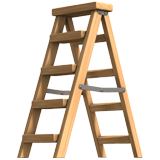
\includegraphics[height=1em]{figs/ladder.png}: Agent improvement with AutoLibra}

AutoLibra can additonally be employed to directly improve agent performance by using extracted metrics to guide targeted modifications to the agent's code, using a human-in-the-loop or another LLM as the editor.

As a demonstration of AutoLibra's capabilities, we present a case study where we use AutoLibra to improve the performance of an agent on baba-is-ai, a highly challenging agentic reasoning task based on the Baba Is You video game. We demonstrate that AutoLibra induces fine-grained, orthogonal [non-redundant], and human-interpretable metrics that have high coverage of the agent's behavior, and show the utility of these metrics in guiding targeted modifications to the agent's to improve its performance and efficiency. We further demonstrate that an agent improved by metrics extracted from AutoLibra outperforms a baseline agent on the task in environment score and trajectory performance, and that the improvements realized by AutoLibra are generalizable to unseen Baba Is You levels and arbitrary LLMs.

\subsection{AutoLibra provides optimization targets for agent prompt engineering}
\label{sec:baba-is-ai}
Baba Is You is a puzzle game in which the player controls a character that can modify the rules of the game by pushing blocks containing words that define the game's rules. Words can be combined to form sentences that define the properties of objects in the game, such as "Baba is You" or "Flag is Win". The goal of the game is to reach a win condition, such as touching a flag, by manipulating the rules of the game to create new win conditions, modify the properties of objects, or change the behavior of the player character.

The game is highly challenging and requires the player to think creatively and reason causally about the game's rules in order to solve the puzzles. This makes Baba Is You an ideal testbed for evaluating the performance of reinforcement learning agents on agentic reasoning tasks; we employ the baba-is-ai environment, a simplified version of Baba Is You \cite{cloos2024babaaibreakrules, paglieri2024balrog} as our testing implementation. Observations of the environment are supplied to the agent in text form, and the agent interacts with the environment by issuing commands in the form of text strings that move the active character.

[Insert figure of baba-is-ai environment]

\subsection{AutoLibra for baba-is-ai improvement}

In performing iterative agent improvement with AutoLibra, a full cycle of the AutoLibra pipeline is considered a full turn, the pseudocode for which is shown in Algorithm 1. One unmodified agent is used as a baseline for comparison (Turn 0), and three complete turns of iterative agent improvement with AutoLibra are performed (Turn 1, 2, 3), for a total of four turns. Six representative tasks for baba-is-ai are used in iterative metric improvement, with the remainder held out for evaluation. The agent is evaluated on the baba-is-ai environment and any changes to the agent code at the beginning of each turn, and the environment score, trajectory performance, and other metrics are recorded at the end of each turn. GPT-4o-241120 is used as the agent model.


\begin{algorithm}
    \caption{Pseudocode for iterative agent improvement with AutoLibra}
    \begin{algorithmic}[1]
    \For{$i$ in range($n\_turns$)}
        \For{$task$ in $selected\_tasks$}
            \State $traj_i, eval\_score_i += agent.play(task, prompt)$
            \State $annotations_i += editor.annotate(traj_i)$
        \EndFor
        \State $metrics_i = AutoLibra.extract_metrics(traj_i, annotations_i)$
        \State $traj\_scores_i = AutoLibra.llm_eval(metrics_i, traj_i)$
        \State $curr\_scores = eval\_score_i$
        \While {$curr\_scores <= eval\_score_i$}
            \State $prompt = updated\_prompt_k$
            \For{$task$ in $selected\_tasks$}
                \State $\_, curr_scores = agent.play(task, prompt)$
            \EndFor
        \EndWhile
    \EndFor

    \end{algorithmic}
\end{algorithm}

\begin{wraptable}[19]{r}{0.60\textwidth} % 'r' for right, adjust the width as needed
\centering
\small
\vspace{-30pt}
\begin{tabular}{ccl}
\toprule
\multicolumn{1}{c}{Emoji}& 
\multicolumn{1}{c}{It.} & 
\multicolumn{1}{l}{Metric} \\
\midrule
\rowcolor{gray!10} 
\includegraphics[scale=0.07]{figs/emojis/emoji_1.png} & 0 & Win Condition Recognition \\
\midrule
\rowcolor{gray!10} 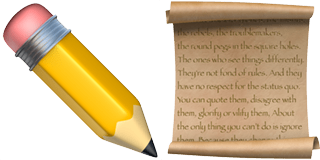
\includegraphics[scale=0.07]{figs/emojis/emoji_2.png} & 0 & Rule Modification \\
\midrule
\rowcolor{gray!10} 
\includegraphics[scale=0.07]{figs/emojis/emoji_3.png} & 0 & Direct Navigation Efficiency \\
\midrule
\rowcolor{gray!10} 
\includegraphics[scale=0.07]{figs/emojis/emoji_4.png} & 0 & Context-Sensitive Decision Making \\
\midrule
\rowcolor{gray!30} 
\includegraphics[scale=0.07]{figs/emojis/emoji_5.png} & 1 & Win Rule Construction \\
\midrule
\rowcolor{gray!30} 
\includegraphics[scale=0.07]{figs/emojis/emoji_6.png} & 1 & Selective Interaction With Relevant Objects  \\
\midrule
\rowcolor{gray!30} 
\includegraphics[scale=0.07]{figs/emojis/emoji_7.png} & 1 & Rule Manipulation and Execution  \\
\midrule
\rowcolor{gray!60} 
\includegraphics[scale=0.07]{figs/emojis/emoji_8.png} & 2 & Subtask Coordination \\
\midrule
\rowcolor{gray!90} 
\includegraphics[scale=0.07]{figs/emojis/emoji_9.png} & 3 & Immovable Interaction \\
\bottomrule
\end{tabular}
\caption{Metrics and Turn of Induction \newline for Baba-Is-AI}
\label{tab:metrics}
\end{wraptable}
\renewcommand{\arraystretch}{1.5} 
\begin{table}[h!]

\centering
\begin{tabular}{|>{\raggedright\arraybackslash}p{6cm}|c|c|c|c|}
\hline
\textbf{Turn} & \textbf{0} & \textbf{1} & \textbf{2} & \textbf{3} \\
\hline
\textbf{Babaisai Score GPT-4o} & 0.30 & 0.40 & 0.43 & 0.55 \\
\hline
\textbf{Babaisai Score Claude 3.5 Sonnet} & 0.35 & 0.40 & 0.45 & 0.55 \\
\hline
\textbf{Average Env. Steps} & 79 & 63 & 60 & 51 \\
\hline
\end{tabular}
\caption{Babaisai Scores and Average Environment Steps}
\end{table}

\subsection{Results}

The induced metrics and the agent's per-task performance are shown in Table \ref{tab:metrics} and Table \ref{tab:heldout}, respectively. A significant improvement in the agent's is observed from Turn 0 to Turn 3, with the agent achieving a both higher environment score and trajectory performance on the held-out tasks compared to the baseline agent. Significantly, the agent's performance on specific metrics increased correspondingly to code changes targeting those metrics, demonstrating the utility of AutoLibra for fine-grained agent improvement. This is discussed in more detail in the following sections.

\subsubsection{Extracted Metrics and Improvements}
The metrics induced by AutoLibra (Table \ref{tab:metrics}) capture the behavior of the agent effectively, with coverage increasing from 65\% at Turn 0 to 92\% at Turn 3 and a low mean redundancy of 56\%. Notably, earlier metrics were found to describe higher-level behaviors than later metrics, reflective of the more complex behaviors that the agent demonstrated in later turns, as well as the compositionality of induced metrics. Code changes were selected to specifically target given metrics, and as seen in Figure \ref{fig:autolibra-training}, the agent's performance on the targeted metric improved significantly in the turn following the code change. This demonstrates the utility of AutoLibra for fine-grained agent improvement, as well as the human interpretability of the induced metrics.

\textbf{Turn 0}
The agent behavior is stochastic and inconsistent, with no clear strategy or goal. Any progress in the environment is the consequence of a random walk. 
\texttt{Win Condition Recognition} 
\includegraphics[scale=0.07]{figs/emojis/emoji_1.png} was identified as a prerequisite to all other metrics induced in this turn, as progress in the environment is impossible without recognizing the win condition, and was therefore targeted for improvement. Improvements took the form of few-shot prompting, by supplying an example of observations and the corresponding win condition and subtasks, and guidance on subtask-level planning, by mapping specific environmental observations to actions that would progress the agent towards the win condition.
\newline
\textbf{Turn 1}
An increase in 
\includegraphics[scale=0.07]{figs/emojis/emoji_1.png} performance of 22\% was observed between Turn 0 and Turn 1, indicating that the code changes were effective in improving the agent's ability to recognize the win condition. A slight but statistically insignificant increase was observed for the other metrics induced in Turn 0, but the agent's overall baba-is-ai environment score increased by 10\%, indicating that 
\includegraphics[scale=0.07]{figs/emojis/emoji_1.png} was correctly identified by AutoLibra as a key bottleneck to the agent's performance in the environment.

The agent now targets specific blocks and objects instead of moving randomly, but gets stuck in loops and on immovable objects, and is unable to consistently complete multi-step tasks.

Based on the metrics induced in Turn 1, several changes to the agent code were implemented:
\begin{itemize}
    \item Augmentation of existing subtask-level planning guidance with low-level position instructions, targeting improvement of \texttt{Rule Modification for Obstacle Management} 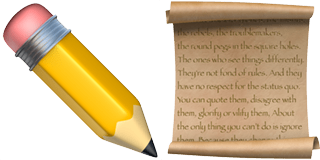
\includegraphics[scale=0.07]{figs/emojis/emoji_2.png} and \texttt{Direct Navigation Efficiency} 
\includegraphics[scale=0.07]{figs/emojis/emoji_3.png}
    \item Meta-prompting \cite{Suzgun_Kalai_2024} by providing subtask identification heuristic, targeting improvement of \texttt{Selective Interaction with Relevant Objects} 
\includegraphics[scale=0.07]{figs/emojis/emoji_6.png} and \texttt{Context-Sensitive Decision Making} 
\includegraphics[scale=0.07]{figs/emojis/emoji_4.png}
    \item Augmentation of single-shot example with movement instructions, targeting improvement of \texttt{Rule Manipulation and Execution} 
\includegraphics[scale=0.07]{figs/emojis/emoji_7.png}
\end{itemize}


\textbf{Turn 2}
Substantial improvements in 
\includegraphics[scale=0.07]{figs/emojis/emoji_1.png} were observed due to more detailed single-shot examples and reasoning templates, and the corresponding increase in other metrics supports idea that 
\includegraphics[scale=0.07]{figs/emojis/emoji_1.png} is a key bottleneck to the agent's performance. We further observed a significant increase in 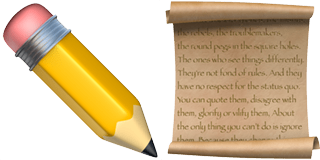
\includegraphics[scale=0.07]{figs/emojis/emoji_2.png} and 
\includegraphics[scale=0.07]{figs/emojis/emoji_7.png}, indicating that the changes targeting these metrics were effective in improving the agent's reasoning performance and consequent avoidance of irrelevant objects. \texttt{Subtask Identification} 
\includegraphics[scale=0.07]{figs/emojis/emoji_5.png} saw no significant improvement, as the agent still misunderstands map directions and confuses rule blocks with objects. 

Qualitatively, the agent now recognizes when wall rules need to be broken and breaks them, but still cannot assemble rules to win, as it gets stuck on immovable blocks and walls and does not understand where rule blocks need to be placed to form a win condition.

Based on the metrics induced in Turn 2, several changes to the agent code were implemented:
\begin{itemize}
    \item Formatting observations as absolute position (as opposed to relative steps from the agent), and listing of immovable/movable blocks to improve \texttt{Direct Navigation Efficiency} 
\includegraphics[scale=0.07]{figs/emojis/emoji_3.png}
    \item Chain-of-thought reasoning to assemble subtask completion agenda based on turn-to-turn observations, targeting improvement of \texttt{Subtask Coordination and Overall Task Planning} 
\includegraphics[scale=0.07]{figs/emojis/emoji_8.png}
    \item Augmentation of single-shot example to few-shot example with reasoning templates, targeting improvement of \texttt{Rule Manipulation and Execution} 
\includegraphics[scale=0.07]{figs/emojis/emoji_7.png}
    \item Explicit instructions on navigation to avoid block collisions and assembly of rules, including movement templates, targeting improvement of \texttt{Rule Manipulation and Execution} 
\includegraphics[scale=0.07]{figs/emojis/emoji_7.png} and \texttt{Win Rule Construction} 
\includegraphics[scale=0.07]{figs/emojis/emoji_5.png}
\end{itemize}

\textbf{Turn 3}
We observe a large increase in 
\includegraphics[scale=0.07]{figs/emojis/emoji_4.png} and \includegraphics[scale=0.07]{figs/emojis/emoji_6.png}, indicating that the changes targeting these metrics were effective in improving the agent's reasoning performance and consequent avoidance of irrelevant objects. \includegraphics[scale=0.07]{figs/emojis/emoji_3.png} saw further improvement, indicating that the use of absolute position and immovable/movable block listing was effective in improving the agent's navigation efficiency. \includegraphics[scale=0.07]{figs/emojis/emoji_7.png} saw a slight increase, indicating that the changes targeting this metric were effective in improving the agent's ability to manipulate rules to achieve the win condition. \includegraphics[scale=0.07]{figs/emojis/emoji_5.png} saw its first improvement, indicating that more complex metrics are effectively targeted when the base performance and simpler metrics are improved.

Qualitatively, nearly agent always understands when wall rule can be and cannot be broken, as well as when it's not necessary to break the wall rule, covers nearly all tasks that involve going to win. The agent understands how to assemble win rules but still struggles with changing block direction and understanding that blocks get stuck against walls

% A turn-by-turn discussion of metrics and targeted code changes is presented in Appendix XXX.
\subsubsection{Held-Out Task Performance}

On the held-out tasks, the agent improved significantly from Turn 0 to Turn 3, with an environment scores of 30\% and 55\%, respectively, a substantial increase compared to the highest base model performance of 33\% on baba-is-ai \cite{paglieri2024balrog}, and demonstrating that the improvements realized by AutoLibra are generalizable to unseen tasks. The agent's trajectory performance also improved significantly, with the average number of steps per task (capped at 100) decreasing from 79 to 51, indicating that the agent's reasoning performance and efficiency improved as a result of the code changes made in each turn. The agent's performance on the held-out tasks is shown in Table \ref{tab:metric_perf}.
%The greatest performance increase was observed between Turn 2 and Turn 3, expected to due to the consistency of wall-breaking and the emergence of rule-construction that was previously absent.


\subsection{Ablation Study}

To evaluate the generalization of the improvements realized by AutoLibra, we conducted an ablation study in which we evaluated the performance of the agent improved by AutoLibra on unseen Baba Is You levels and arbitrary LLMs.

\subsubsection{Different LLMs}

The agent code for each turn (0-3) was tested with Claude-3-5 instead of GPT-4o-241120, and the agent's performance was evaluated on the baba-is-ai environment. Table XXX shows that the agent's performance was found to be consistent across all turns, with no significant difference in environment score or trajectory performance observed between the two LLMs. This demonstrates that the improvements realized by AutoLibra are generalizable to arbitrary LLMs, and that the induced metrics are robust to changes in the underlying LLM.

\subsubsection{Different Environment}

AutoLibra was further evaluated in a new environment, whose rules and objectives were different from those of baba-is-ai. MiniHack is a grid navigation game expressed in text similar to baba-is-ai, consisting of a procedurally generated environment that requires the agent to navigate a space consisting of various agent roles, creatures, items, and tasks to reach a goal \cite{samvelyan2021minihackplanetsandboxopenended}. Given its plasticity and abundant elements, MiniHack is more challenging and diversified than baba-is-ai as it can simulate significantly different environments that test different capabilities of agents. Similar as our experiments with baba-is-ai, the improvement for MiniHack also follows Algorithm 1. Two turns of iterative agent improvement with AutoLibra were performed on MiniHack. Four representative tasks for MiniHack are used in iterative metric improvement, with the remainder held out for evaluation. The agent is evaluated on the MiniHack environment and any changes to the agent code at the beginning of each turn, and the environment score, trajectory performance, and other metrics are recorded at the end of each turn. GPT-4o-241120 is used as the agent model.\\
\\
\begin{figure}[ht]
    \centering
    \includegraphics[width=\textwidth]{figs/emojis/maps.png}
    \caption{Overview of four maps used in the agent optimization process. 
    From left to right, up to down: (1) \emph{Boxoban}, (2) \emph{MazeWalk}, (3) \emph{Corridor Fight}, and (4) \emph{Quest}.}
    \label{fig:minihack_maps}
\end{figure}


\begin{table}[ht]
\centering
\begin{tabular}{|c|c|l|}
\hline
\textbf{} & \textbf{Turn} & \textbf{Description} \\
\hline
\rowcolor{gray!10} \includegraphics[scale=0.07]{figs/emojis/mini_1.png} & 0 & Target Navigation Effectiveness \\
\hline
\rowcolor{gray!10} \includegraphics[scale=0.07]{figs/emojis/mini_2.png} & 0 & Efficient Exploration and Map Memory Utilization \\
\hline
\rowcolor{gray!10} \includegraphics[scale=0.07]{figs/emojis/mini_3.png} & 0 & Hazard Awareness and Equipment Utilization \\
\hline
\rowcolor{gray!10} \includegraphics[scale=0.07]{figs/emojis/mini_4.png} & 0 & Boulder Manipulation Strategy \\
\hline
\rowcolor{gray!10} \includegraphics[scale=0.07]{figs/emojis/mini_5.png} & 0 & Combat Engagement and Survival \\
\hline
\rowcolor{gray!10} \includegraphics[scale=0.07]{figs/emojis/mini_6.png} & 0 & Role-Specific Ability Utilization  \\
\hline
\rowcolor{gray!30} \includegraphics[scale=0.07]{figs/emojis/mini_7.png} & 1 & Spatial Awareness and Interpretation  \\
\hline
\rowcolor{gray!30} \includegraphics[scale=0.07]{figs/emojis/mini_8.png} & 1 & Object Pickup Efficiency \\
\hline
\rowcolor{gray!60} \includegraphics[scale=0.07]{figs/emojis/mini_9.png} & 2 & Giant Rats Encounter Handling \\
\hline
\end{tabular}
\caption{Metrics and Turn of Introduction for MiniHack}
\label{tab:metrics_mini}
\end{table}


\renewcommand{\arraystretch}{1.5} 
\begin{table}[h!]

\centering
\begin{tabular}{|>{\raggedright\arraybackslash}p{6cm}|c|c|c|}
\hline
\textbf{Turn} & \textbf{0} & \textbf{1} & \textbf{2} \\
\hline
\textbf{MiniHack Score GPT-4o} & 0.00 & 0.125 & 0.25 \\
\hline
\textbf{Average Env. Steps} & 85.00 & 91.13 & 88.5 \\
\hline
\end{tabular}
\caption{MiniHack Score and Average Environment Steps}
\label{tab:heldout_mini}
\end{table}

\subsubsection{Representative Tasks}
The four selected representative tasks each provide a unique perspective on evaluating an agent's capability. Figure \ref{fig:minihack_maps} shows an example for each task, and from left to right, up to down, these maps respectively represent Boxoban, MazeWalk, Corridor Fight, and Quest. Boxoban is a box-pushing game inspired by Sokoban. To succeed in Boxoban, the agent needs to push the four boulders(orange balls) onto the four fountains(blue icons), and partial credit will be awarded for pushing some of the boulders onto the fountains. Boxoban tests the agent's capability in strategic planning and rule-following. MazeWalk is a game that requires the agent to explore unknown dark spaces to find the target downstairs(the icon with a downward arrow). Two challenges for MazeWalk are invisibility—the agent has a highly restrained vision of the map in the beginning—and darkness—even if the agent has visited a block, the block will plunge into darkness as the agent walks away. Thus, MazeWalk tests the agent's capability in map memory and strategic searching. Corridor Fight is a game that requires the agent to explore the unknown dark corridor to find the target downstairs while surviving the giant rats. Corridor Fight tests the agent's capability in memory, space awareness, hazard awareness, and strategic combat. Finally, Quest requires the agent to use a tool to help itself cross the deadly lava, survive randomly generated monsters, and search for the target downstairs. As the most randomized game, it tests the agent's abilities to recognize and utilize tools, understand its role and special power, and strategically survive from monsters.


\subsubsection{Results}

The induced metrics and the agent's per-task performance are shown in Table \ref{tab:metrics_mini}, Table \ref{tab:metric_mini_perf}, respectively. A substantial improvement in the agent's is observed from Turn 1 to Turn 2, with the agent achieving a both higher environment score and trajectory performance on the held-out tasks compared to the baseline agent. Specifically, the agent's performance on specific metrics increased correspondingly to prompt changes targeting those metrics, demonstrating the utility of AutoLibra for fine-grained agent improvement. This is discussed in more detail in the following sections.


\paragraph{\textit{4.4.4.1 Extracted Metrics and Improvements}}~\newline 
\\The metrics induced by AutoLibra (Table \ref{tab:metrics_mini}) capture the behavior of the agent effectively through all turns, with coverage of 83\% at Turn 0 to 88\% at Turn 2 and a low average redundancy of 66\%. Notably, due to the diversity of tasks, most metrics only focus on one or two tasks. Moreover, the metrics generated at turn 0 are already complete enough as they show a good coverage of all four tasks, and the later metrics were found to describe detailed behaviors for targeting one task respectively. Prompt changes were selected to specifically target given metrics, and as seen in Figure \ref{fig:autolibra-training}, the agent's performance on the targeted metric improved significantly in the turn following the code change. This demonstrates the utility of AutoLibra for fine-grained agent improvement, as well as the human interpretability of the induced metrics.


\paragraph{\textit{4.4.4.2 Held-Out Task Performance}}~\newline 
\\For the held-out tasks, the agent improved from turn 0 to turn 2, with score from 0\% to 25\%, respectively, a substantial increase compared to the highest base model performance of 33\% on baba-is-ai \cite{paglieri2024balrog}, and demonstrating that the improvements realized by AutoLibra are generalizable to unseen tasks. The agent's trajectory performance also improved significantly, with the average number of steps per task (capped at 100) decreasing from 79 to 51, indicating that the agent's reasoning performance and efficiency improved as a result of the code changes made in each turn. The agent's performance on the held-out tasks is shown in Table \ref{tab:metric_perf}.



\subsection{Style}

Papers to be submitted to COLM 2025 must be prepared according to the
instructions presented here.

%% Please note that we have introduced automatic line number generation
%% into the style file for \LaTeXe. This is to help reviewers
%% refer to specific lines of the paper when they make their comments. Please do
%% NOT refer to these line numbers in your paper as they will be removed from the
%% style file for the final version of accepted papers.

Authors are required to use the COLM \LaTeX{} style files obtainable at the
COLM website. Please make sure you use the current files and
not previous versions. Tweaking the style files may be grounds for rejection.

\subsubsection{Copy Options}

If your paper is ultimately accepted, the option {\tt
  {\textbackslash}final} should be set  for the {\tt {\textbackslash}usepackage[submission]\{colm2025\_conference\}} command for the camera ready version. The {\tt submission} options is the default, and is to be used for all submissions during the review process. It also turns on the line numbers. If you wish to submit a preprint, the option {\tt preprint} should be used.
  
  

\subsection{Retrieval of style files}

The style files for COLM and other conference information are available online at:
\begin{center}
   \url{http://www.colmweb.org/}
\end{center}
The file \verb+colm2025_conference.pdf+ contains these
instructions and illustrates the
various formatting requirements your COLM paper must satisfy.
Submissions must be made using \LaTeX{} and the style files
\verb+colm2025_conference.sty+ and \verb+colm2025_conference.bst+ (to be used with \LaTeX{}2e). The file
\verb+colm2025_conference.tex+ may be used as a ``shell'' for writing your paper. All you
have to do is replace the author, title, abstract, and text of the paper with
your own.

The formatting instructions contained in these style files are summarized in
sections \ref{gen_inst}, \ref{headings}, and \ref{others} below.

\section{General formatting instructions}
\label{gen_inst}

The text must be confined within a rectangle 5.5~inches (33~picas) wide and
9~inches (54~picas) long. The left margin is 1.5~inch (9~picas).
Use 10~point type with a vertical spacing of 11~points. Palatino is the
preferred typeface throughout, and is mandatory for the main text. Paragraphs are separated by 1/2~line space, with no indentation. 

Paper title is 17~point and left-aligned.
All pages should start at 1~inch (6~picas) from the top of the page.

Please verify that any custom header information you may add does not override the style defined in this document. This has been known to occur especially when submissions are converted to a new template from a previous one (i.e., for re-submission to a different venue). 

Authors' names are
set in boldface, and each name is placed above its corresponding
address. The lead author's name is to be listed first, and
the co-authors' names are set to follow. Authors sharing the
same address can be on the same line.

Please pay special attention to the instructions in section \ref{others}
regarding figures, tables, acknowledgements, and references.


There will be a strict upper limit of 9 pages for the main text of the initial submission, with unlimited additional pages for citations. 

We strongly recommend following arXiv's guidelines for making your paper friendly for HTML conversion: \url{https://info.arxiv.org/help/submit_latex_best_practices.html}.


\section{Headings: first level}
\label{headings}

First level headings are in lower case (except for first word and proper nouns), bold face,
flush left and in point size 12. One line space before the first level
heading and 1/2~line space after the first level heading.

\subsection{Headings: second level}

Second level headings are in lower case (except for first word and proper nouns), bold face,
flush left and in point size 10. One line space before the second level
heading and 1/2~line space after the second level heading.

\subsubsection{Headings: third level}

Third level headings are in lower case (except for first word and proper nouns), bold face, italics, 
flush left and in point size 10. One line space before the third level
heading and 1/2~line space after the third level heading.

\section{Citations, figures, tables, references}\label{others}

These instructions apply to everyone, regardless of the formatter being used.

\subsection{Citations within the text}

Citations within the text should be based on the \texttt{natbib} package
and include the authors' last names and year (with the ``et~al.'' construct
for more than two authors). When the authors or the publication are
included in the sentence, the citation should not be in parenthesis using \verb|\citet{}| (as
in ``See \citet{Vaswani+2017} for more information.''). Otherwise, the citation
should be in parenthesis using \verb|\citep{}| (as in ``Transformers are a key tool
for developing language models~\citep{Vaswani+2017}.'').

The corresponding references are to be listed in alphabetical order of
authors, in the \textsc{References} section. As to the format of the
references themselves, any style is acceptable as long as it is used
consistently.

\subsection{Footnotes}

Indicate footnotes with a number\footnote{Sample of the first footnote} in the
text. Place the footnotes at the bottom of the page on which they appear.
Precede the footnote with a horizontal rule of 2~inches
(12~picas).\footnote{Sample of the second footnote}

\subsection{Figures}

All artwork must be neat, clean, and legible. Lines should be dark
enough for purposes of reproduction; art work should not be
hand-drawn. Any text within the figure must be readable. We ask to not use font sizes below {\tt small}. We strongly recommend to use vector representations (e.g., pdf or svg) for all diagrams. 
We strongly recommend positioning all figures at the top or bottom of the page.

The figure number and caption always appear below the figure. Place one line space before the figure caption, and one line space after the figure. The figure caption is lower case (except for first word and proper nouns); figures are numbered consecutively.
Make sure the figure caption does not get separated from the figure.
Leave sufficient space to avoid splitting the figure and figure caption.

You may use color figures.
However, it is best for the
figure captions and the paper body to make sense if the paper is printed
either in black/white or in color.
\begin{figure}[t]
\begin{center}
%\framebox[4.0in]{$\;$}
\fbox{\rule[-.5cm]{0cm}{4cm} \rule[-.5cm]{4cm}{0cm}}
\end{center}
\caption{Sample figure caption.}
\end{figure}

\subsection{Tables}

All tables must be centered, neat, clean and legible. Do not use hand-drawn tables. The table number and title always appear below the table. See Table~\ref{sample-table}. Please do not use font sizes below {\tt small} in tables. We recommend using {\tt booktabs} or a similar package to style tables. 
We strongly recommend positioning all tables at the top or bottom of the page.

Place one line space before the table title, one line space after the table title, and one line space after the table. The table title must be lowercase (except for first word and proper nouns); tables are numbered consecutively.

\begin{table}[t]
\begin{center}
\begin{tabular}{ll}
\toprule
\multicolumn{1}{c}{\bf PART}  &\multicolumn{1}{c}{\bf DESCRIPTION} \\
\midrule
Dendrite         &Input terminal \\
Axon             &Output terminal \\
Soma             &Cell body (contains cell nucleus) \\
\bottomrule
\end{tabular}
\end{center}
\caption{Sample table title}\label{sample-table}
\end{table}




\section{Final instructions}
Do not change any aspects of the formatting parameters in the style files.
In particular, do not modify the width or length of the rectangle the text
should fit into, and do not change font sizes (except perhaps in the
\textsc{References} section; see below). Please note that pages should be
numbered.

\section{Preparing PostScript or PDF files}

Please prepare PostScript or PDF files with paper size ``US Letter'', and
not, for example, ``A4''. The -t
letter option on dvips will produce US Letter files.

Consider directly generating PDF files using \verb+pdflatex+
(especially if you are a MiKTeX user).
PDF figures must be substituted for EPS figures, however.

Otherwise, please generate your PostScript and PDF files with the following commands:
\begin{verbatim}
dvips mypaper.dvi -t letter -Ppdf -G0 -o mypaper.ps
ps2pdf mypaper.ps mypaper.pdf
\end{verbatim}

\subsection{Margins in LaTeX}

Most of the margin problems come from figures positioned by hand using
\verb+\special+ or other commands. We suggest using the command
\verb+\includegraphics+
from the graphicx package. Always specify the figure width as a multiple of
the line width as in the example below using .eps graphics
\begin{verbatim}
   \usepackage[dvips]{graphicx} ...
   \includegraphics[width=0.8\linewidth]{myfile.eps}
\end{verbatim}
or % Apr 2009 addition
\begin{verbatim}
   \usepackage[pdftex]{graphicx} ...
   \includegraphics[width=0.8\linewidth]{myfile.pdf}
\end{verbatim}
for .pdf graphics.
See section~4.4 in the graphics bundle documentation (\url{http://www.ctan.org/tex-archive/macros/latex/required/graphics/grfguide.ps})

A number of width problems arise when LaTeX cannot properly hyphenate a
line. Please give LaTeX hyphenation hints using the \verb+\-+ command.

\section*{Author Contributions}
If you'd like to, you may include  a section for author contributions as is done
in many journals. This is optional and at the discretion of the authors.

\section*{Acknowledgments}
Use unnumbered first level headings for the acknowledgments. All
acknowledgments, including those to funding agencies, go at the end of the paper.

\section*{Ethics Statement}
Authors can add an optional ethics statement to the paper. 
For papers that touch on ethical issues, this section will be evaluated as part of the review process. The ethics statement should come at the end of the paper. It does not count toward the page limit, but should not be more than 1 page. 



\bibliography{colm2025_conference}
\bibliographystyle{colm2025_conference}

\appendix
\section{Appendix}
You may include other additional sections here.

\end{document}
